\documentclass[10pt,a4paper]{article}

%%%%%%%%%%%%%%%%%%%%%%%%%%%
% MODIFY:

\newcommand{\authorA}{Ahmad Bin Qasim (03693345)}
\newcommand{\authorB}{Kaan Atukalp (03709123)}
\newcommand{\authorC}{Martin Meinel (03710370)}
\newcommand{\groupNumber}{H} % - YOUR GROUP NUMBER
\newcommand{\exerciseNumber}{3} % - THE NUMBER OF THE EXERCISE
\newcommand{\sourceCodeLink}{https://gitlab.lrz.de/ga53rog/praktikum-ml-crowd}

\newcommand{\workPerAuthor}{
\authorA&Task 1&33\%\\
      &Task 2&33\%\\
      &Task 3&33\%\\
      &Task 4&33\%\\
      &Task 5&33\%\\
      \hline
\authorB&Task 1&33\%\\
      &Task 2&33\%\\
      &Task 3&33\%\\
      &Task 4&33\%\\
      &Task 5&33\%\\
      \hline
\authorC&Task 1&33\%\\
      &Task 2&33\%\\
      &Task 3&33\%\\
      &Task 4&33\%\\
      &Task 5&33\%\\
}

%%%%%%%%%%%%%%%%%%%%%%%%%%%

%%
% imports for the exercise sheets
%

\usepackage[utf8]{inputenc}
\usepackage{amsmath}
\usepackage{amsfonts}
\usepackage{amssymb}

\usepackage[yyyymmdd]{datetime}
\renewcommand{\dateseparator}{--}

\usepackage[left=2cm,right=2cm,top=3cm,bottom=3cm]{geometry}

\usepackage{hyperref}

\usepackage{amsthm}
\newtheorem{lem}{Lemma}
\newtheorem{thm}{Theorem}
\newtheorem{cor}{Corollary}
\newtheorem{rem}{Remark}
\newtheorem{definition}{Definition}
\newtheorem{ter}{Terminology}

\usepackage{graphicx}

\newcommand{\M}{\mathcal{M}}
\newcommand{\N}{\mathcal{N}}
\newcommand{\K}{\mathcal{K}}
\newcommand{\SPDk}{\mathbb{P}^k}
\newcommand{\vol}{\text{vol}}

\newcommand{\Figref}[1]{Figure~\ref{#1}}
\newcommand{\figref}[1]{figure~\ref{#1}}
\newcommand{\Eqnref}[1]{Equation~(\eqref{#1})}
\newcommand{\eqnref}[1]{equation~(\eqref{#1})}

\usepackage{float}
\usepackage{tabularx}
\usepackage{subcaption}
\usepackage{mwe}

\usepackage{fancyhdr}
\pagestyle{fancy}

\usepackage{totcount}
\newtotcounter{taskCounter}
\newtotcounter{pointCounter}
\newenvironment{task}[1]{\noindent\stepcounter{taskCounter}\textbf{Report on task #1}\smallbreak\hrule\smallbreak}{\smallbreak\hrule\bigbreak}


\title{Report for exercise \exerciseNumber~from group~\groupNumber}

\makeatletter
\let\thetitle\@title
\let\theauthor\@author
\let\thedate\@date
\makeatother

\providecommand{\versiondate}{\today}

\lhead{Exercise sheet \exerciseNumber}
\chead{Master Praktikum: Modelling and Simulation of Crowds WS2019/20}
\rhead{TUM}
\lfoot{Report of Group \groupNumber}
\cfoot{\thepage}
\rfoot{Last compiled: \versiondate}
\renewcommand{\headrulewidth}{0.4pt}
\renewcommand{\footrulewidth}{0.4pt}

\newcommand{\frontpage}{
\begin{center}
\textbf{\thetitle}\\~\\
\end{center}
\begin{table}[H]
\begin{tabular}{ll}
Tasks addressed:&\total{taskCounter}\\
Authors:&\authorA\\
&\authorB\\
&\authorC\\
Last compiled:&\versiondate\\
Source code:&\sourceCodeLink
\end{tabular}
\end{table}
\vfill
The work on tasks was divided in the following way:
\begin{table}[H]
\begin{tabularx}{\textwidth}{X|p{2cm}|p{2cm}}
\workPerAuthor
\end{tabularx}
\end{table}
\newpage
}

\begin{document}

\frontpage

\begin{task}{1, Vector fields, orbits, and visualization}
A phase portrait is a good way to visualize a dynamical system with a one or two-dimensional state space. The linear dynamical system is defined with a state space $X = \mathbb{R}, I = \mathbb{R}$, parameter $\alpha \in \mathbb{R}$ and flow $\phi_{\alpha}$ defined by $\frac{\partial \phi_{\alpha}(t,x)}{\partial t}|_{t=0} = A_{\alpha}x$ with $A_{\alpha} = \begin{bmatrix}\alpha&\alpha \\ -\frac{1}{4}&0\end{bmatrix}$. The task is to adjust $\alpha$ in the parametric matrix A to create phase portraits of a node, saddle and focus. Afterwards it has to be specified if the different systems for the different alphas are topologically equivalent or not. The phase portrait of a dynamical system depends on how the derivative of its flow looks like. In general you can distinguish between five topological classes of hyperbolic equilibria on the plane.
\begin{itemize}
    \item If you have two negative eigenvalues and no positive eigenvalue without any imaginary parts the phase portrait will be classified as a stable node, where the lines point in direction of the node.
    \item The dynamical system is still stable for the case that there are only negative eigenvalues but without any imaginary part. In this case the phase portrait changes to a stable focus. Stable foci and stable nodes are topologically equivalent.
    \item In case there is one negative and one positive eigenvalue the system is not stable anymore. The phase portrait is classified as a saddle.
    \item If both eigenvalues are positive and do not have any imaginary part then the phase diagram can be classified as a node. It is an unstable node, because only systems with only negative eigenvalues are stable.
    \item The last case is if a system has two positive eigenvalues with an imaginary part. This leads to an unstable focus. As for the stable focus and stable node the unstable focus and unstable node are topologically equivalent.
\end{itemize}
The goal of this task is to choose different values for $\alpha$ in order to generate all these different five phase plots. We compute the eigenvalues by computing: \begin{align*}
    det(A_\alpha - \lambda I) \overset{!}{=} 0 \\
    (\alpha -\lambda)(-\lambda) - (-\frac{1}{4}\alpha) \overset{!}{=}0\\
    \lambda^2-\alpha \lambda + \frac{1}{4}\alpha \overset{!}{=}0\\
    \lambda_{1/2} = \frac{\alpha (+/-) \sqrt{\alpha^2-\alpha}}{2}
\end{align*}
The equation for $\lambda_1 =  \frac{\alpha + \sqrt{\alpha^2-\alpha}}{2}$ is always $> 0$. Consequently there will never be the case that both eigenvalues are negative. As a consequence of this the system can be seen as unstable. We have to find three different values for $\alpha$ to obtain a saddle, an unstable focus and an unstable node. For the value of $alpha = 2$ there are two positive eigenvalues: $\lambda_1 = 1.71$ and $\lambda_2 = 0.29$. The phase diagram is an unstable node which can be seen in Figure \ref{fig:task1_node}.
\begin{figure}[H]
    \centering
    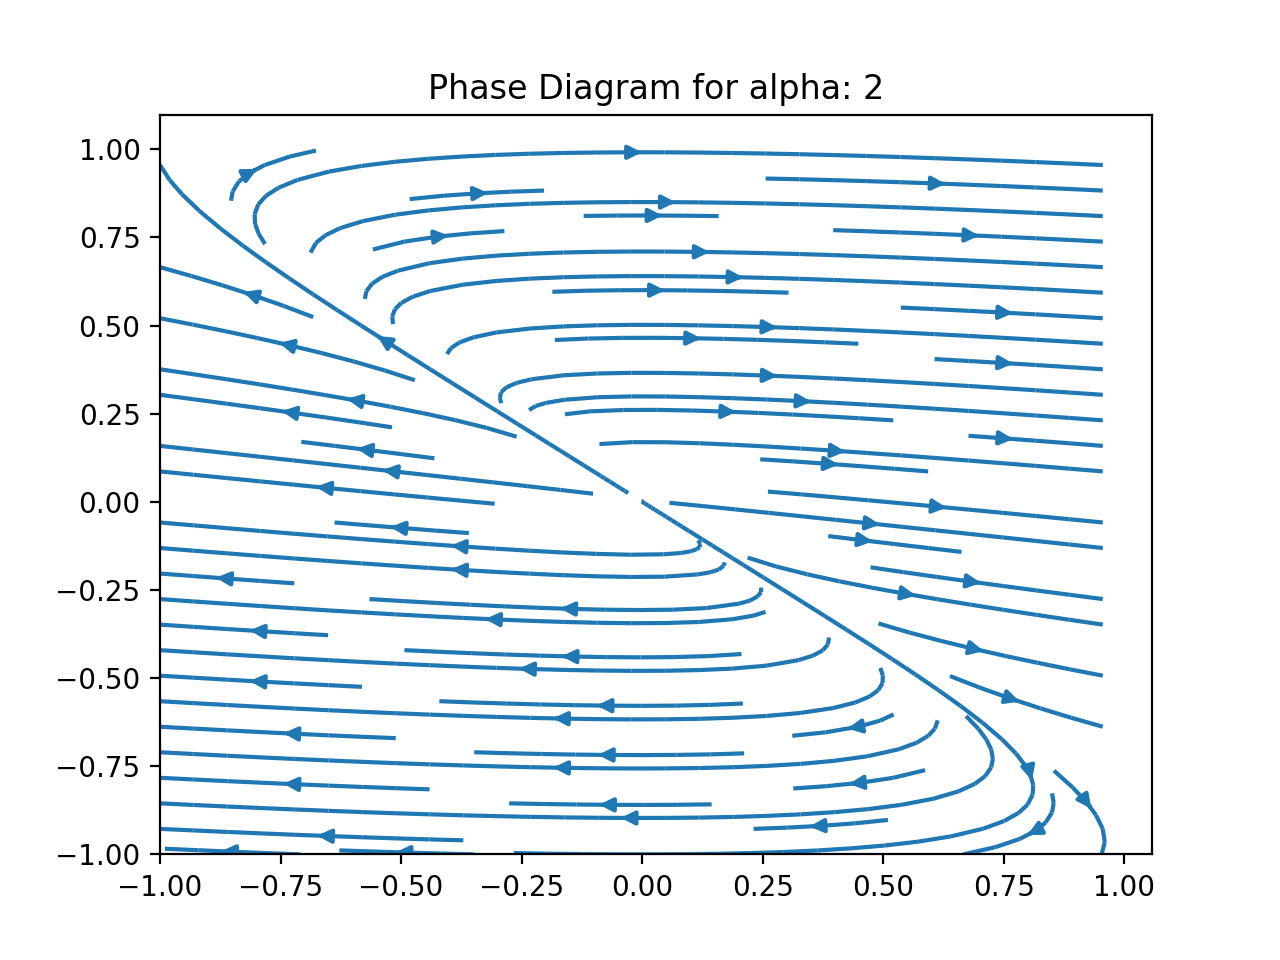
\includegraphics[width=0.7\textwidth]{../plots/node.png}
    \caption{Phase diagram showing a node for two positive eigenvalues and $\alpha = 2$}
    \label{fig:task1_node}
\end{figure}
We choose an $\alpha = 0.5$ to obtain two positive eigenvalues with imaginary part. These two eigenvalues are $\lambda_{1/2} = \frac{0.5 (+/-) 0.5i}{2}$. These eigenvalues lead to an unstable focus, which can be seen in Figure
\begin{figure}[H]
    \centering
    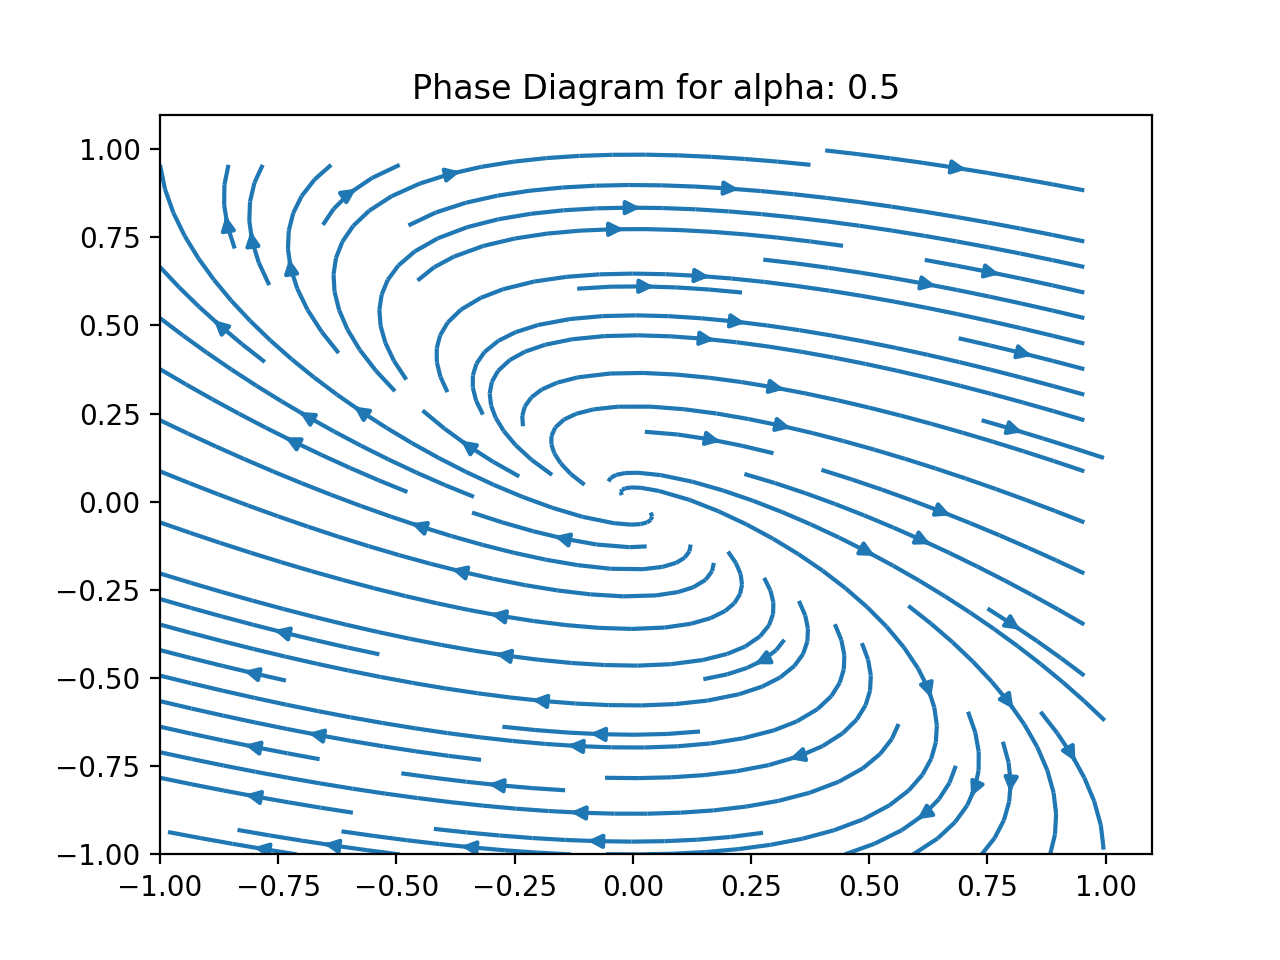
\includegraphics[width=0.7\textwidth]{../plots/focus.png}
    \caption{Phase diagram showing a focus for two positive eigenvalues with imaginary part for $\alpha = \frac{1}{2}$}
    \label{fig:task1_focus}
\end{figure}
A value of $\alpha=-0.1$ leads to the two eigenvalues $\lambda_1 = 0.11$ and $\lambda_2=-0.22$. One eigenvalue is positive and the other negative. This leads to an unstable saddle which is shown by Figure \ref{fig:task1_saddle}.
\begin{figure}[H]
    \centering
    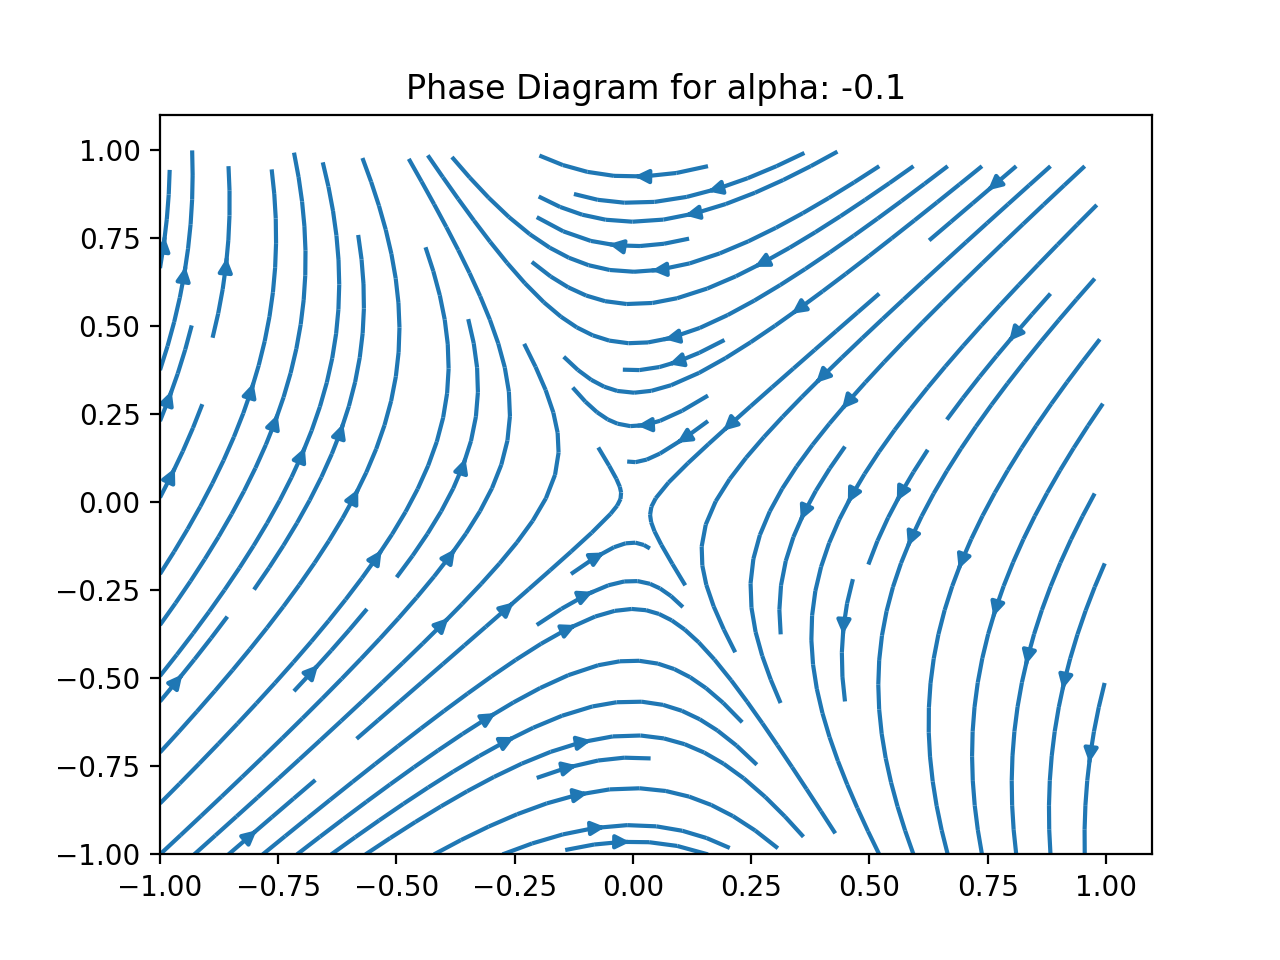
\includegraphics[width=0.7\textwidth]{../plots/saddle.png}
    \caption{Phase diagram showing a saddle for one positive and one negative eigenvalue for $\alpha = -0.1$}
    \label{fig:task1_saddle}
\end{figure}
In general foci and nodes are topologically equivalent if both are stable or both are unstable. Consequently the phase diagrams shown by Figure \ref{fig:task1_focus} and \ref{fig:task1_node} are topologically equivalent, because both of them are unstable. \cite{Kuznetsov:1998:EAB:289919}
\end{task}
\begin{task}{2, Common bifurcations in nonlinear systems}
     \begin{figure}[H]
        \centering
        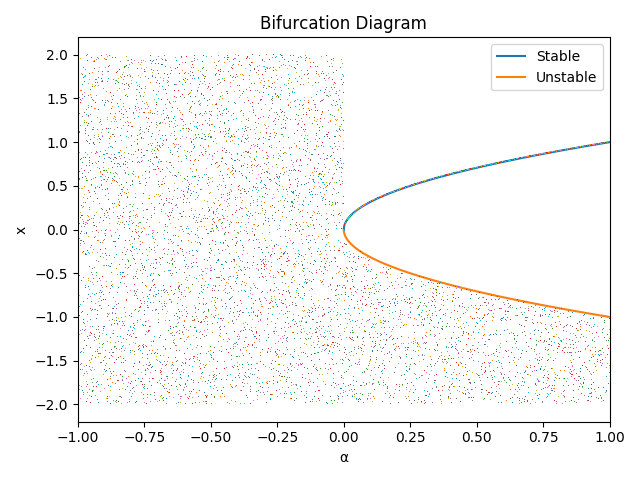
\includegraphics[width=0.6\textwidth]{../plots/task2_1.png}
        \caption{The bifurcation diagram for equation 6 with $\alpha$ in (-1,1)}
        \label{fig:task2_1_bifurcation}
    \end{figure}    
    \begin{figure}[H]
        \centering
        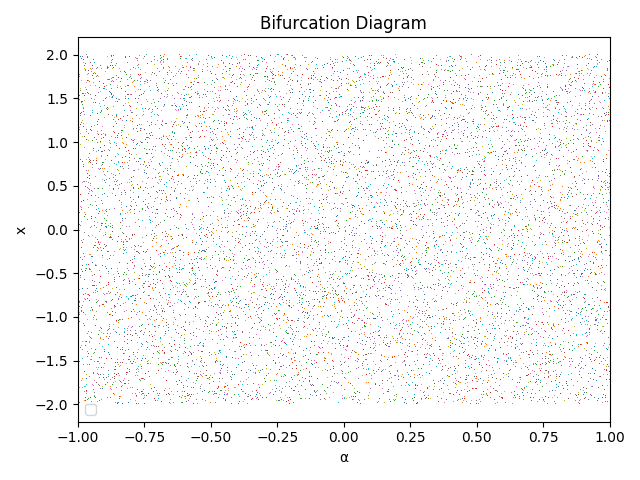
\includegraphics[width=0.6\textwidth]{../plots/task2_2.png}
        \caption{The bifurcation diagram for equation 7 with $\alpha$ in (-1,1)}
        \label{fig:task2_2_bifurcation}
    \end{figure}
	
	We know that, for two dynamical systems to be topologically equivalent, there should exist homeomorphism of the parameter space and a parameter-dependent homeomorphism of the phase space.
	
	\begin{enumerate}
		\item The bifurcation that occurs at $\alpha=0$ is, saddle node bifurcation.
		\item The dynamical systems explained by equation 6 and 7 are not topologically equivalent for $\alpha=1$ because, although they have the same normal form. The dynamical system explained by equation 7 has no steady state for $\alpha=1$, instead the steady state of the dynamical system in question exists at $x0 = \pm \sqrt{\frac{\alpha -2}{2}}$ only for $\alpha > 2$ as shown by figure \ref{fig:task2_3_bifurcation}. According to the definition of topological equivalence mentioned before, for $\alpha=1$ the parameter-dependent homeomorphism of the phase space does not exist.
		\item The dynamical systems explained by equation 6 and 7 are not topologically equivalent for $\alpha=-1$ as well, because at $\alpha=-1$ neither of the dynamical systems have any steady states.
	\end{enumerate}	        
    
    \begin{figure}[H]
        \centering
        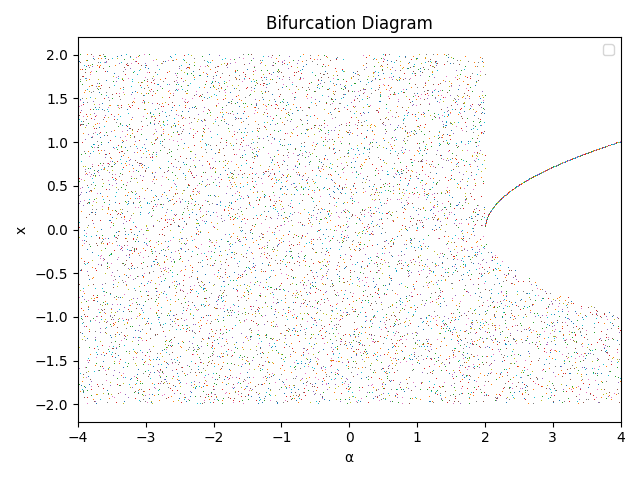
\includegraphics[width=0.6\textwidth]{../plots/task2_3.png}
        \caption{The bifurcation diagram for equation 7 with $\alpha$ in (-4,4)}
        \label{fig:task2_3_bifurcation}
    \end{figure}
\end{task}
\begin{task}{3, Bifurcations in higher dimensions}
The Andronov-Hopf bifurcation is an important bifurcation for systems with one parameter and two-dimensional state spaces. The vector field in normal form is defined by the following equations:
\begin{align*}
    \dot{x_1} &= \alpha x_1 - x_2-x_1(x_1^2+x_2)^2\\ 
    \dot{x_2}&=x_1+\alpha x_2 -x_2(x_1^2+x_2)^2
\end{align*}
The following phase diagrams  show the bifurcation of the system for three different values for $alpha$.
\begin{figure}[H]
    \centering
    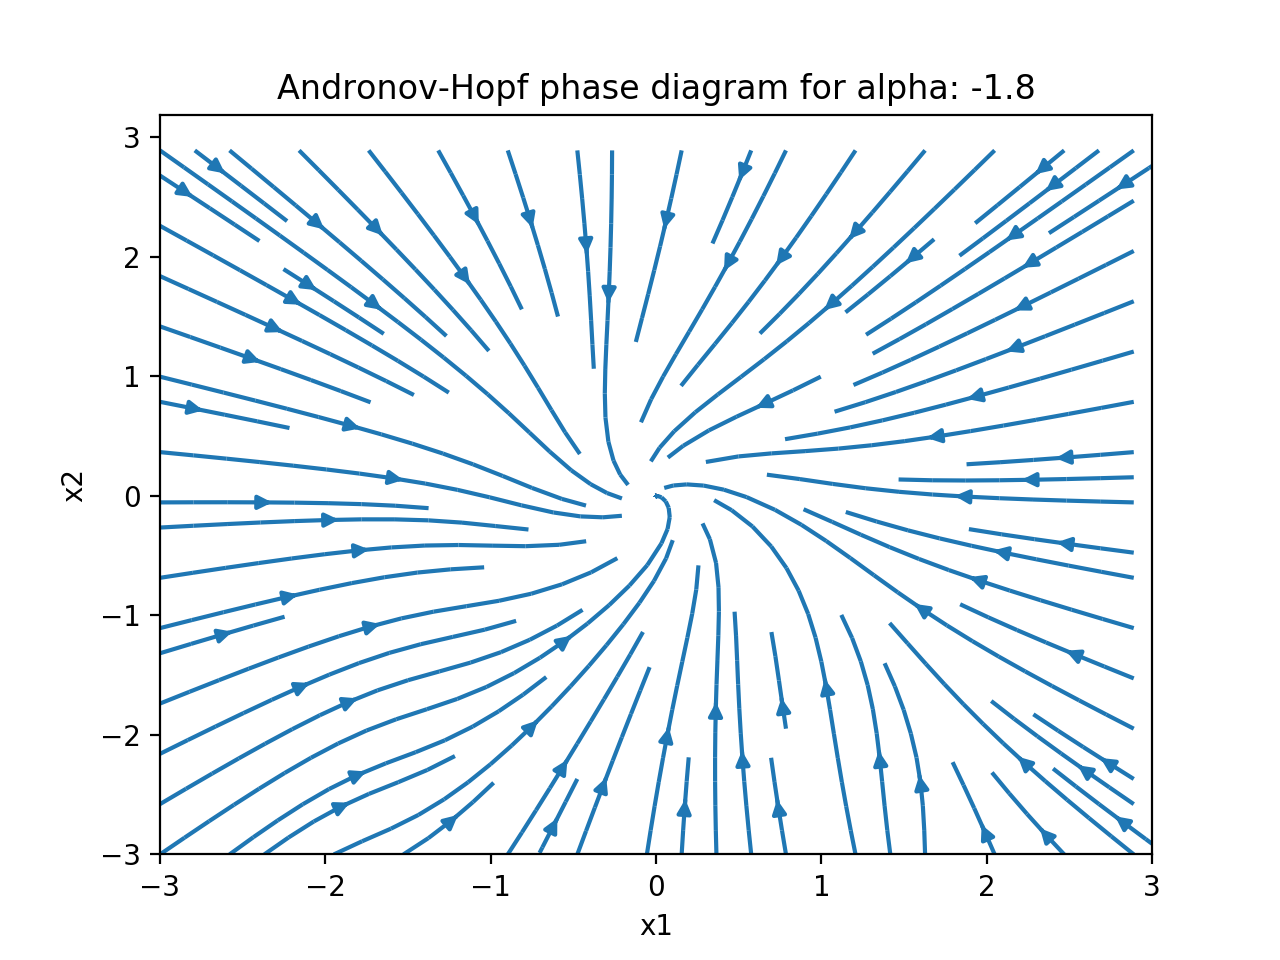
\includegraphics[width=0.7\textwidth]{../plots/Andronov_1,8.png}
    \caption{Phase diagram for Andronov-Hopf bifurcation for $\alpha = -1.8$}
    \label{fig:task3_-1.8}
\end{figure}
\begin{figure}[H]
    \centering
    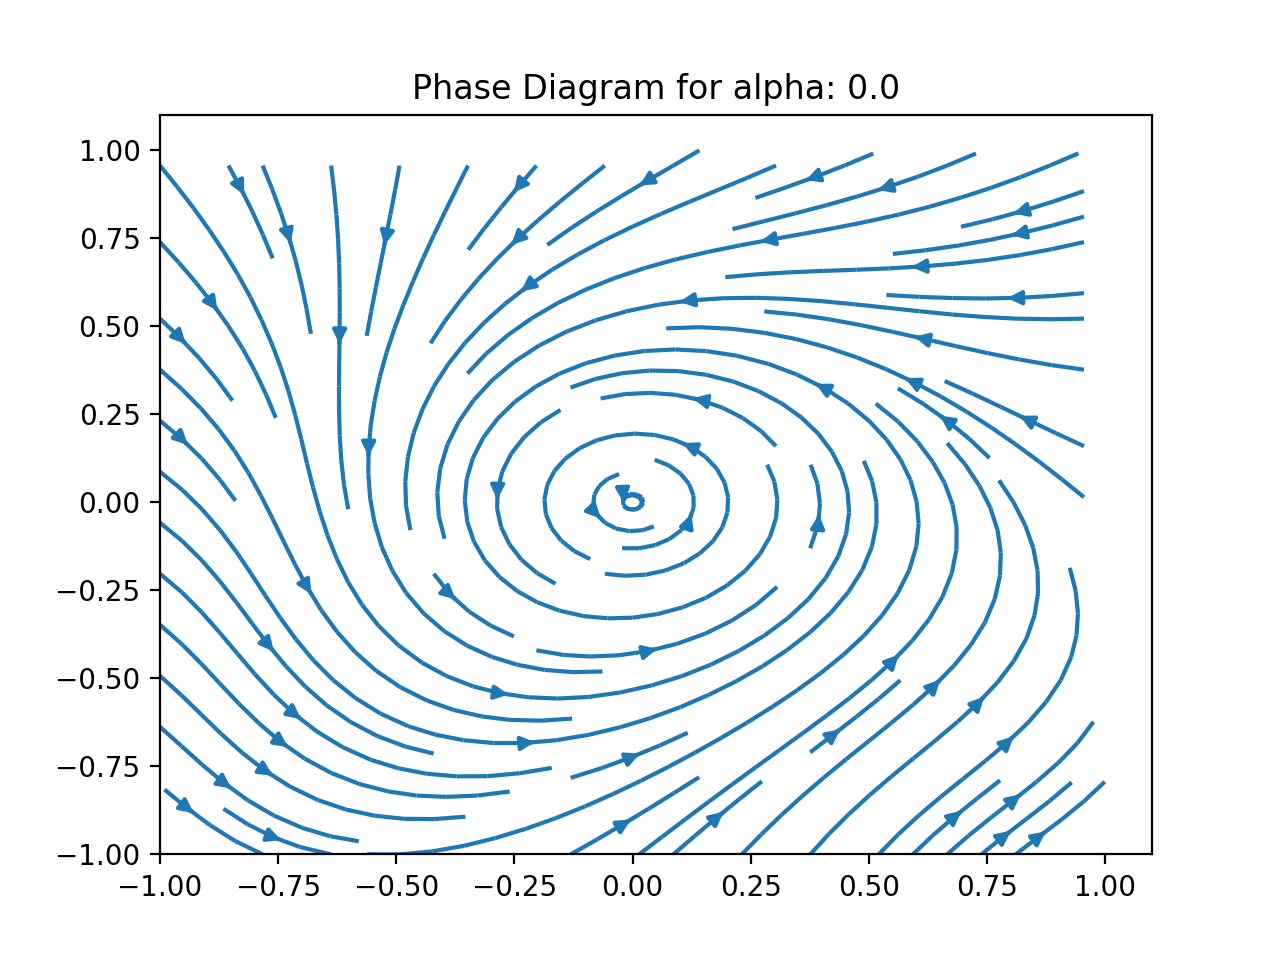
\includegraphics[width=0.7\textwidth]{../plots/Andronov_0.png}
    \caption{Phase diagram for Andronov-Hopf bifurcation for $\alpha=0.0$}
    \label{fig:task3_0.0}
\end{figure}
\begin{figure}[H]
    \centering
    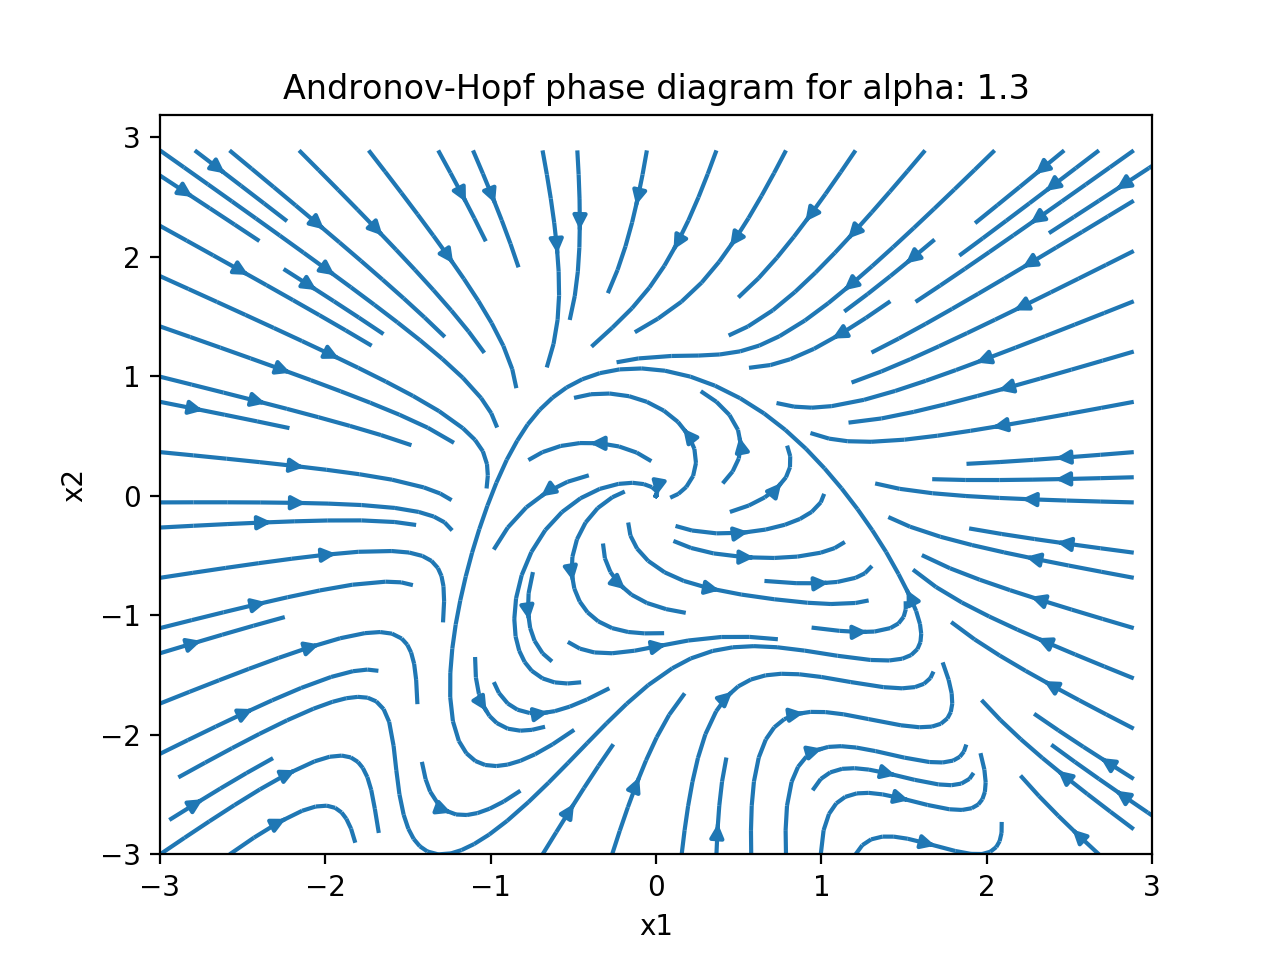
\includegraphics[width=0.7\textwidth]{../plots/Andronov_1,3.png}
    \caption{Phase diagram for Andronov-Hopf bifurcation for $\alpha =1.3 $}
    \label{fig:task3_1.3}
\end{figure}
The figures show that the stability of the equilibrium changes when the value for $\alpha$ changes from negative to positive. This can be seen if the direction of the arrows are compared between Figure \ref{fig:task3_-1.8} and Figure \ref{fig:task3_1.3}. Furthermore a unique limit cycle builds when $\alpha$ passes through zero and the equilibrium changes stability. This cycle can be seen in Figure \ref{fig:task3_1.3}.\\
Besides we computed and visualized two orbits of the system forward in time for the starting points (2,0) and (0.5,0) and a fixed value for $\alpha = 1$. The Euler's method is used to predict the next coordinates of the orbit. The Euler's method computes the next coordinates for an orbit as follows:
\begin{equation*}
    x_n = x_{n-1} + \delta t * v(x_{n-1})
\end{equation*}
We use the Andronov-Hopf bifurcation, because of that v(x) corresponds to the equations for $\dot{x_1} $and$\dot{x_2}$ which are shown above. Furthermore we use a small value of $\delta t = 0.01$. The starting point is marked in green, while the end point is marked in blue for the following figures. Figure \ref{fig:task3_orbit2} shows the orbit for starting at the point of $\begin{bmatrix} 2.0\\0.0\end{bmatrix}$ which is marked in green and ending at the point marked in blue. It can be seen that the ending point is not a stable point. This means that from starting at the point $\begin{bmatrix} 2.0\\0.0\end{bmatrix}$ it will never converge to a stable point it will always go around on its orbit as it did several times which can be seen in Figure \ref{fig:task3_orbit2}. Figure \ref{fig:task3_orbit0.5} shows the orbit for starting at $\begin{bmatrix} 0.5\\0.0\end{bmatrix}$, but it shows as well that the same applies for this orbit as for the orbit before. There is not a stalbe point where the point converges to after a certain amount of steps. It will not stop moving. It will always stay on its orbit and walk on it. This behaviour is visualized in Figure \ref{fig:task3_orbit0.5}, where the starting point is marked in green again and the end point in blue. As already mentioned this is not a stable endpoint, because the point will not stop to move forward at a certain point.
\begin{figure}[H]
    \centering
    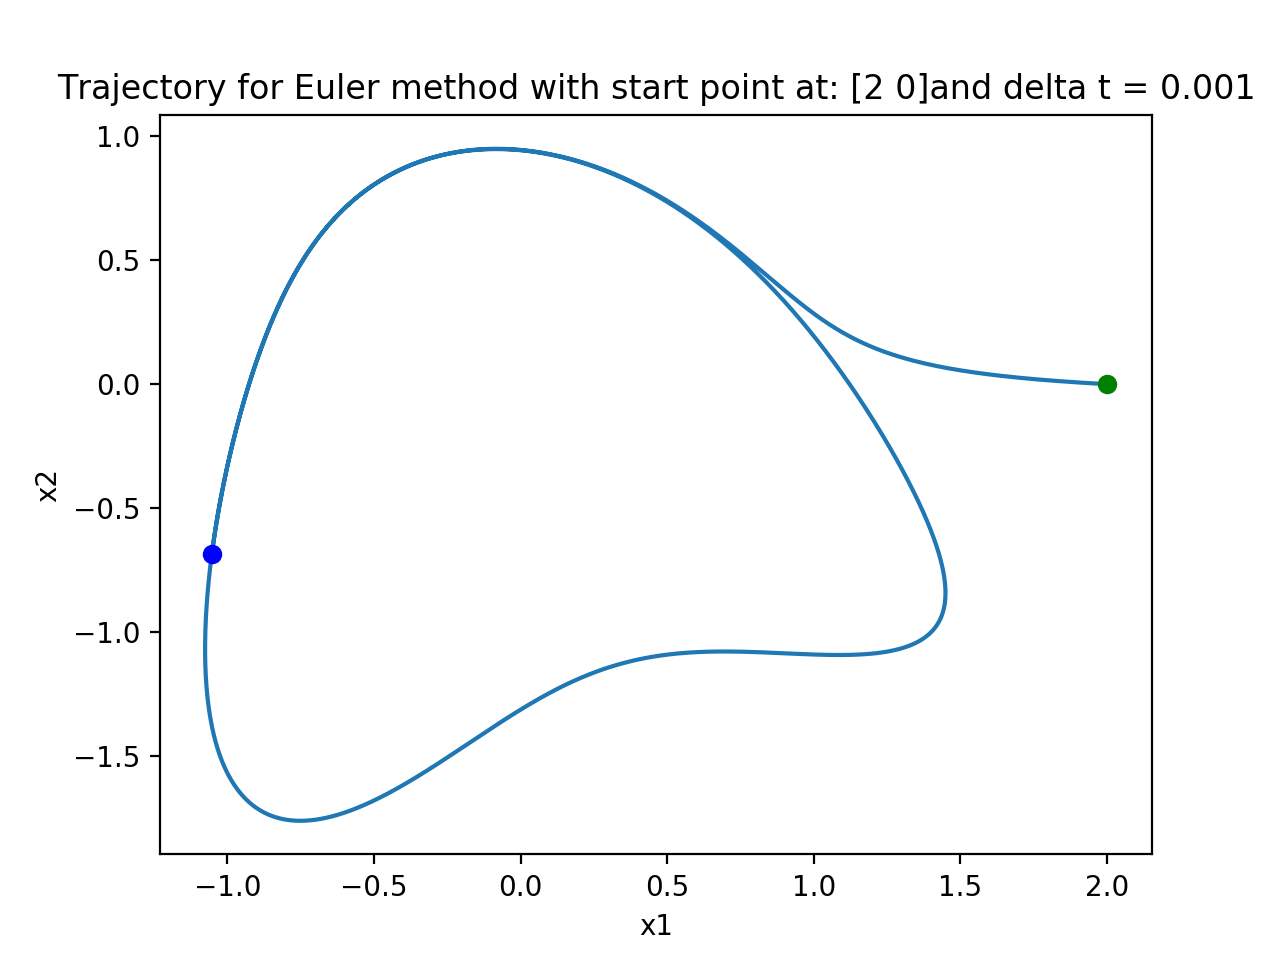
\includegraphics[width=0.7\textwidth]{../plots/Figure_3.png}
    \caption{Orbit for starting at (2.0,0.0) using Euler's method}
    \label{fig:task3_orbit2}
\end{figure}
\begin{figure}[H]
    \centering
    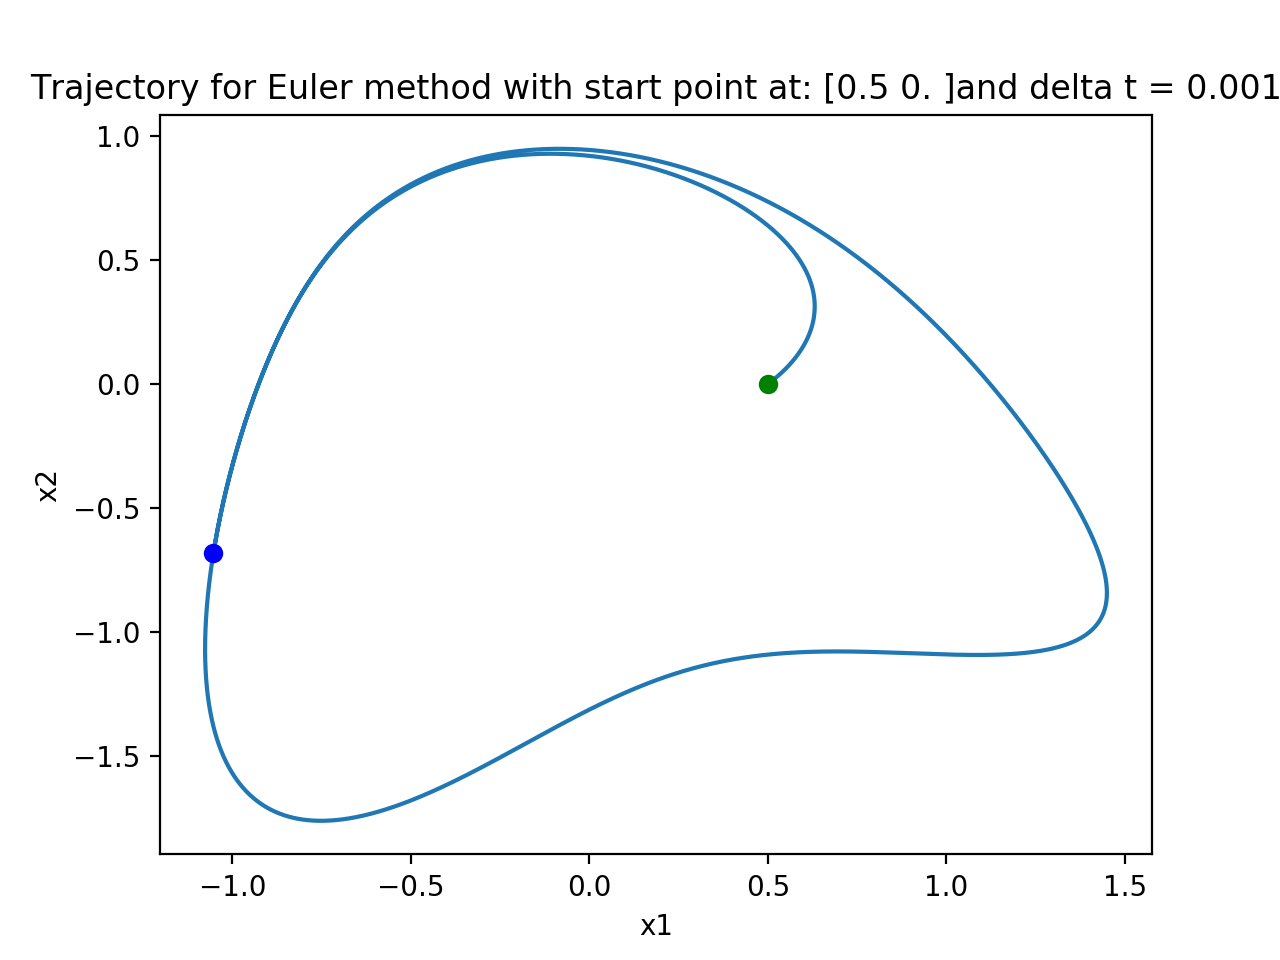
\includegraphics[width=0.7\textwidth]{../plots/Figure_4.png}
    \caption{Orbit for starting at (0.5,0.0) using Euler's method}
    \label{fig:task3_orbit0.5}
\end{figure}
\bigbreak
The cusp bifurcation occurs already in one state space dimension $X=\mathbb{R}$, but with two parameters $\alpha \in \mathbb{R}^2$. The normal form of the cusp bifurcation is given with:
\begin{equation*}
    \dot{x} = \alpha_1 + \alpha_2x - x^3
\end{equation*}
The bifurcation surface, where $\dot{x} = 0$ is visualized in Figure \ref{fig:task3_cusp}. It is called cusp bifurcation, because it fulfills the following cusp bifurcation conditions (1, 2). \\
\begin{equation}
     \lambda = f_x(0,0) = 0 
\end{equation}
\begin{equation}
     b = \frac{1}{2}f_{xx}(0,0) = 0
\end{equation}
You can see that both conditions are fulfilled if you plug in $x = 0$, $\alpha_1 = 0$ and $\alpha_2 = 0$ into both equations. The functions for $f_x(x,\alpha)$ and $f_{xx}(x,\alpha)$ are given below. Consequently f has for $\alpha=0$ the equilibrium $x= 0$. This is characteristic for cusp bifurcation. \cite{Kuznetsov:1998:EAB:289919}
\begin{align*}
    \dot{x} = f(x,\alpha), x\in \mathbb{R}, \alpha \in \mathbb{R}^2 \\
    f_x(x,\alpha) = \alpha_2 - 6x^2 \\
    f_{xx}(x,\alpha) = -12x 
\end{align*}
\begin{figure}[H]
    \centering
    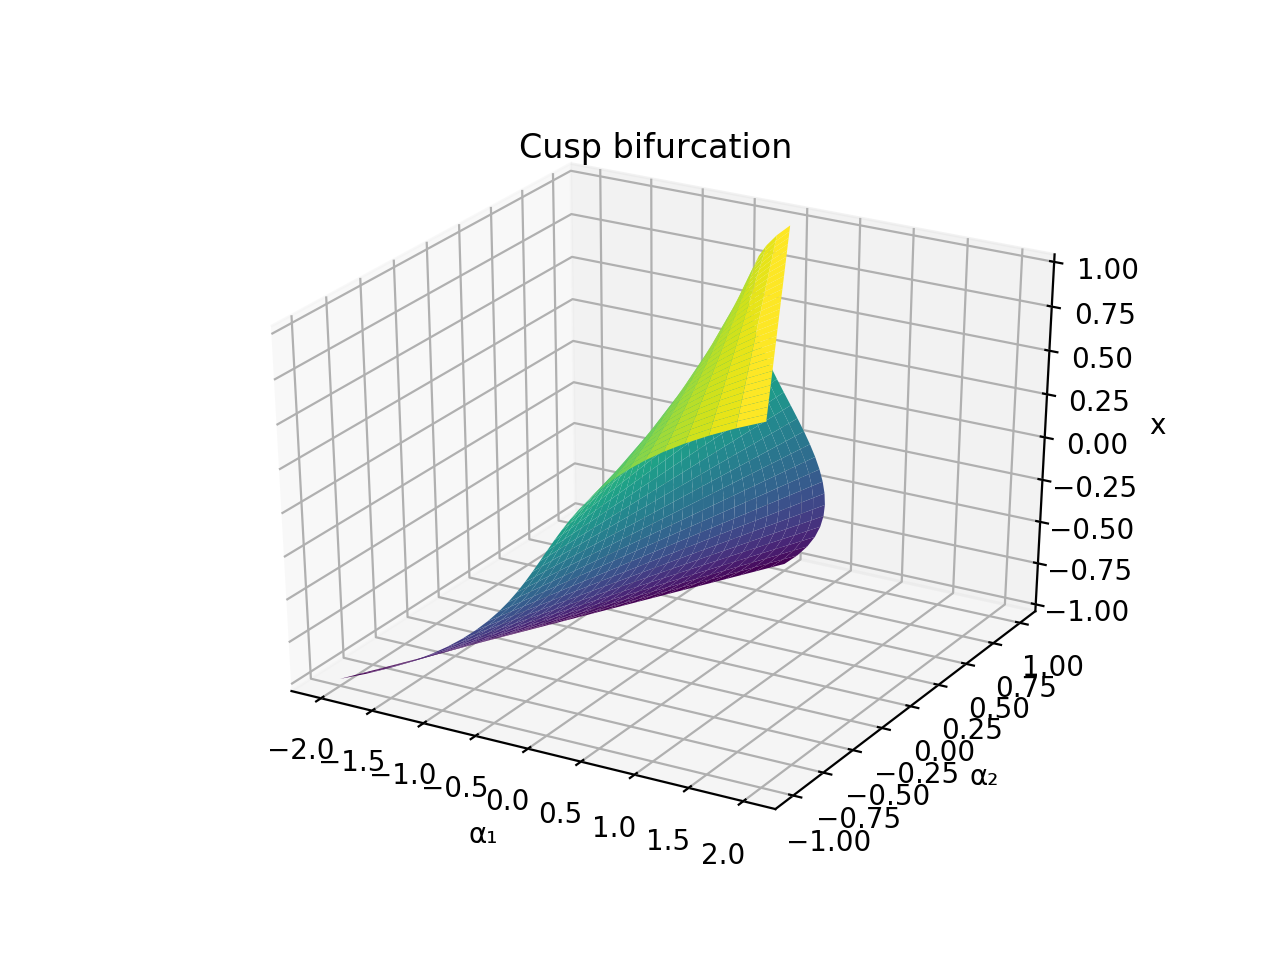
\includegraphics[width=0.7\textwidth]{../plots/Figure_0.png}
    \caption{Cusp bifurcation surface}
    \label{fig:task3_cusp}
\end{figure}
\end{task}
\begin{task}{4, Chaotic dynamics}
For a bifurcation analysis, a random x value between 0 and 1 is chosen and iterated 120 times and then the following 60 iteration coordinates are saved. The evolution equation is as follows: \\
\begin{equation}
    x_{n+1}= r x_n (1 - x_n), n \in \mathbb{N}
\end{equation}

No bifurcations occur and there is a steady state for all r values between 0 and 2 (see Figure \ref{fig:logistic_bif_02}). The steady state is $x=0$ for all $r<1$ since r values are constantly multiplied with each other at every iteration. Period-doubling bifurcations start to happen around $r=3$ and there are still steady states until $r=3.567$ (see Figure \ref{fig:logistic_bif_24}). Except for some values in between ($x = 2.63, 3.74, 3.83$), there are limit cycles with an increasing range as r increases. When r=4, the limit cycle is roughly within range $[0, 1]$ as seen in Figure \ref{fig:logistic_bif_04}. \\

\begin{figure}[H]
    \centering
    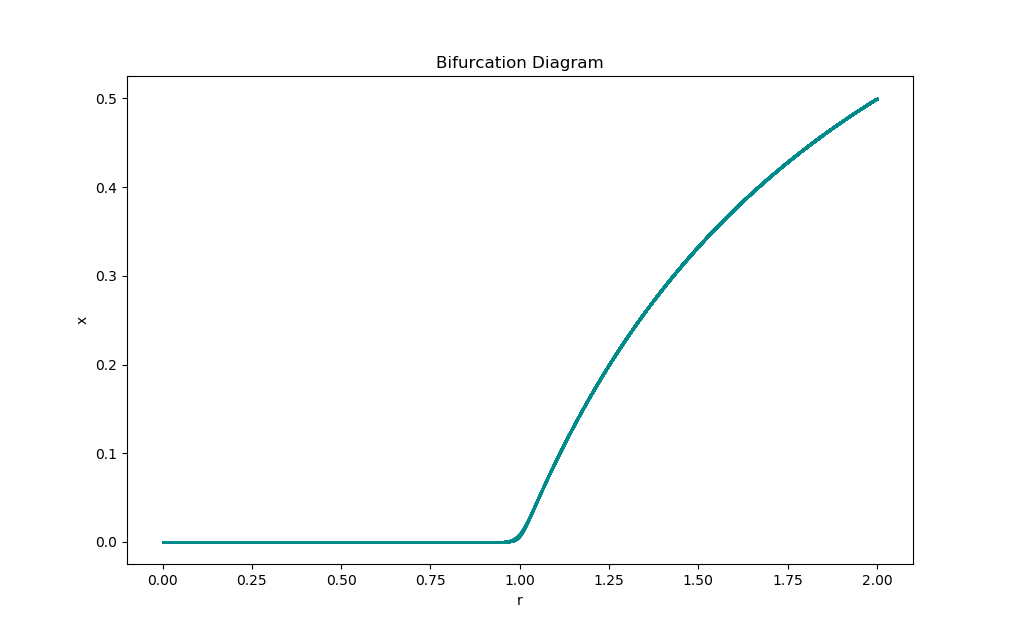
\includegraphics[width=0.7\textwidth]{../plots/logistic_bif_0-2.png}
    \caption{Bifurcation diagram of the logistic map between $r$ values of $0$ and $2$.}
    \label{fig:logistic_bif_02}
\end{figure}

\begin{figure}[H]
    \centering
    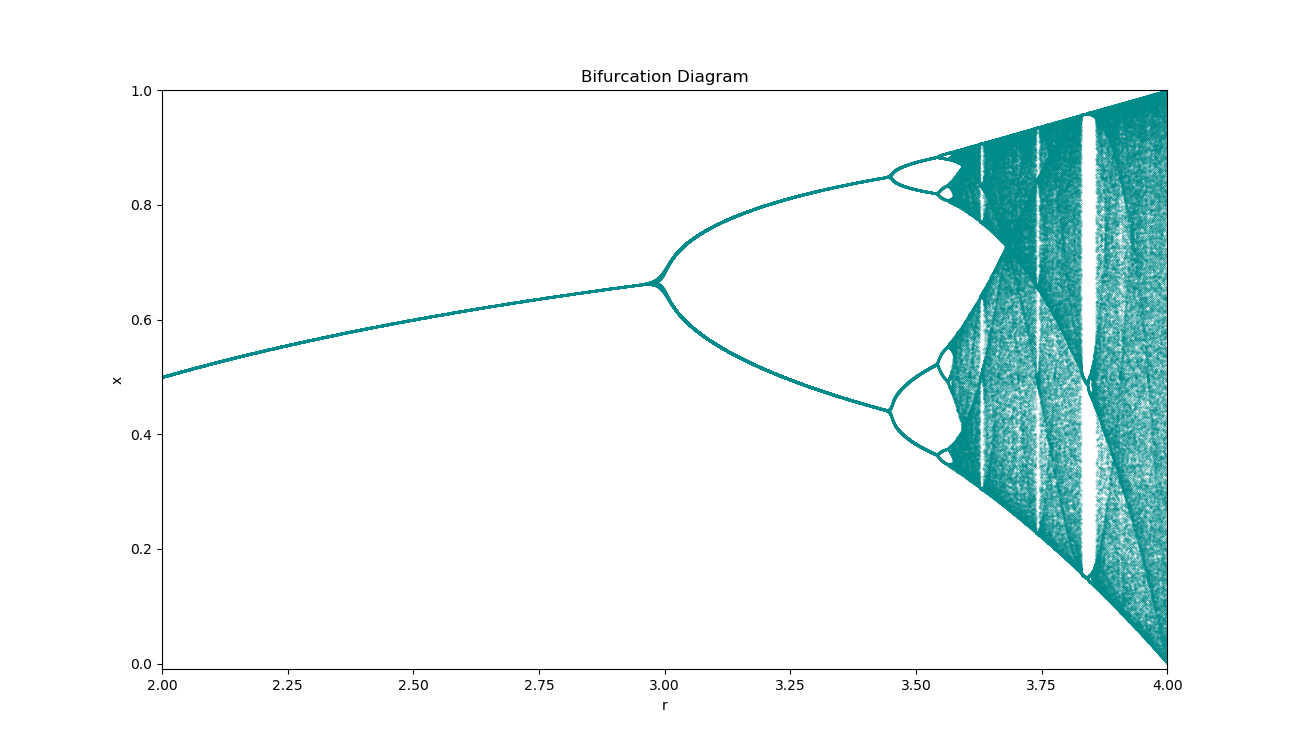
\includegraphics[width=0.7\textwidth]{../plots/logistic_bif_2-4.png}
    \caption{Bifurcation diagram of the logistic map between $r$ values of $2$ and $4$.}
    \label{fig:logistic_bif_24}
\end{figure}

\begin{figure}[H]
    \centering
    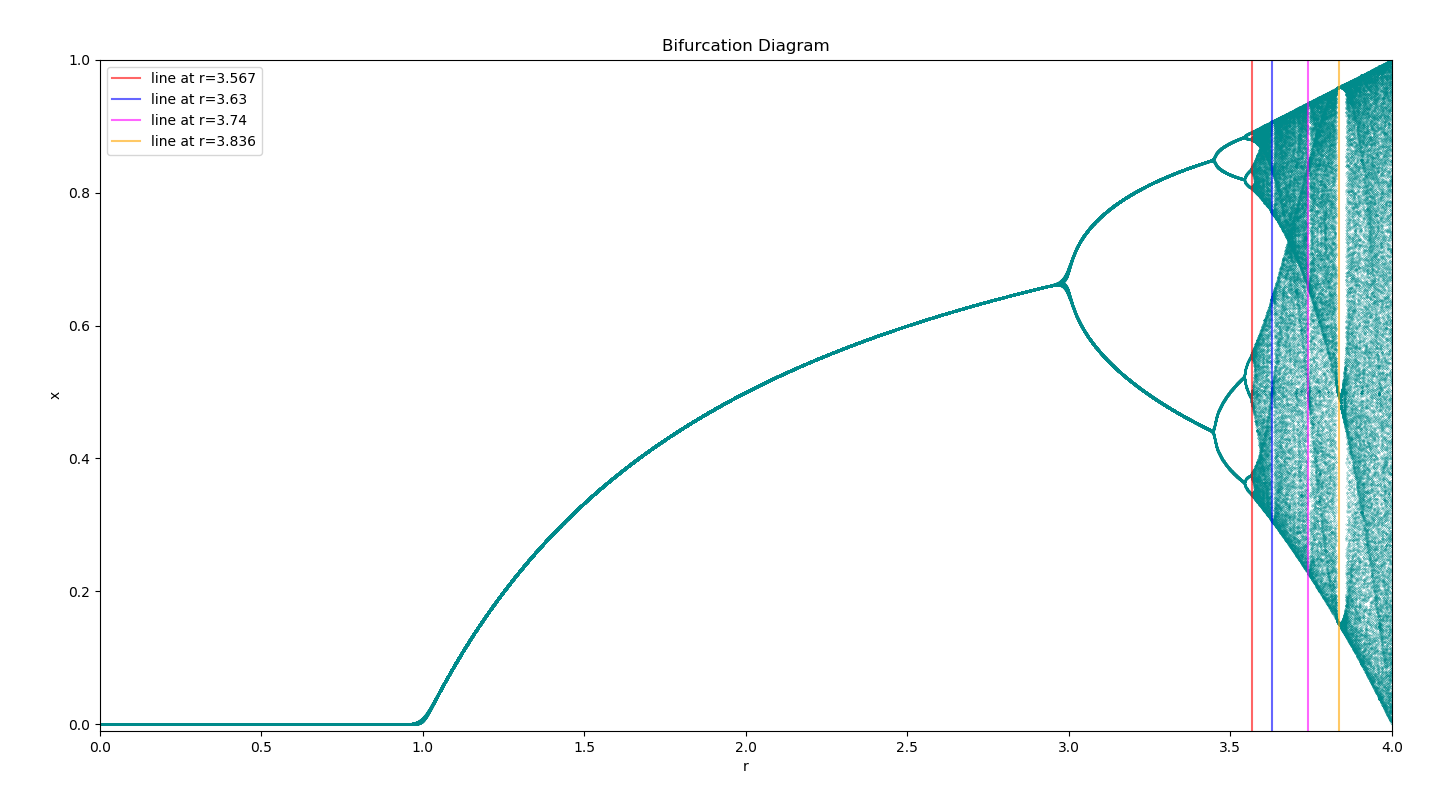
\includegraphics[width=0.7\textwidth]{../plots/logistic_bif_0-4.png}
    \caption{Bifurcation diagram of the logistic map between $r$ values of $0$ and $4$. Vertical lines indicate the steady states.}
    \label{fig:logistic_bif_04}
\end{figure}

The trajectories of a Lorenz system of parameters $\alpha=10$, $\beta=8/3$, and $\rho=28$ until $T=1000$ with the starting points $(10, 10, 10)$ and $(10+10^{-8}, 10, 10)$ were calculated and plotted using the \texttt{solve\_ivp} method of Python’s \texttt{scipy} module. The trajectory looks like a butterfly as seen in Figures \ref{fig:lorenz_1} and \ref{fig:lorenz_2}. The chaotic nature of the system can be realised when these two trajectories are plotted together (see Figure \ref{fig:lorenz_3}). The trajectories are quite non-overlapping even though the starting points were extremely close to each other. The distances between the trajectories are less than 1 only for the $T$ values from $0$ until $23$ and $T$ values of $25$, $608$, $609$, and $654$ within the first 1000 time steps. \\

\begin{figure}[H]
    \centering
    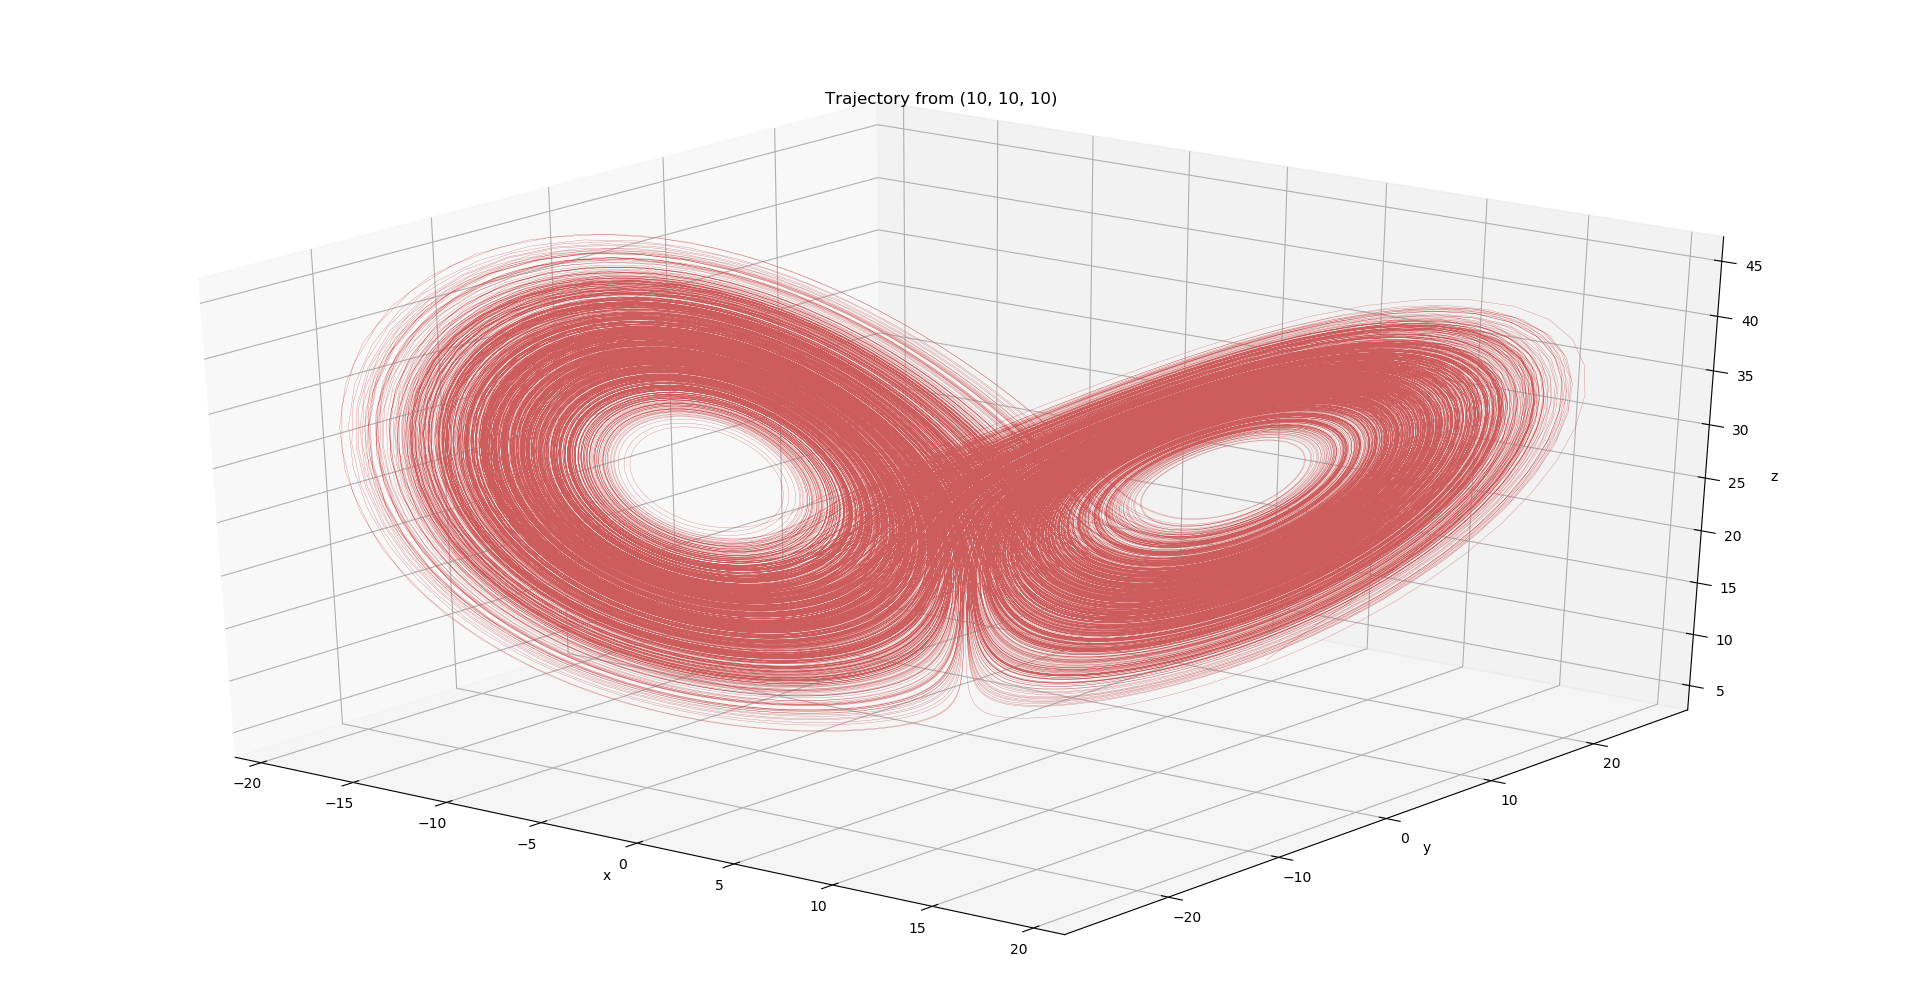
\includegraphics[width=0.7\textwidth]{../plots/lorenz_1.png}
    \caption{The trajectory of a Lorenz system with starting point $(10, 10, 10)$.}
    \label{fig:lorenz_1}
\end{figure}

\begin{figure}[H]
    \centering
    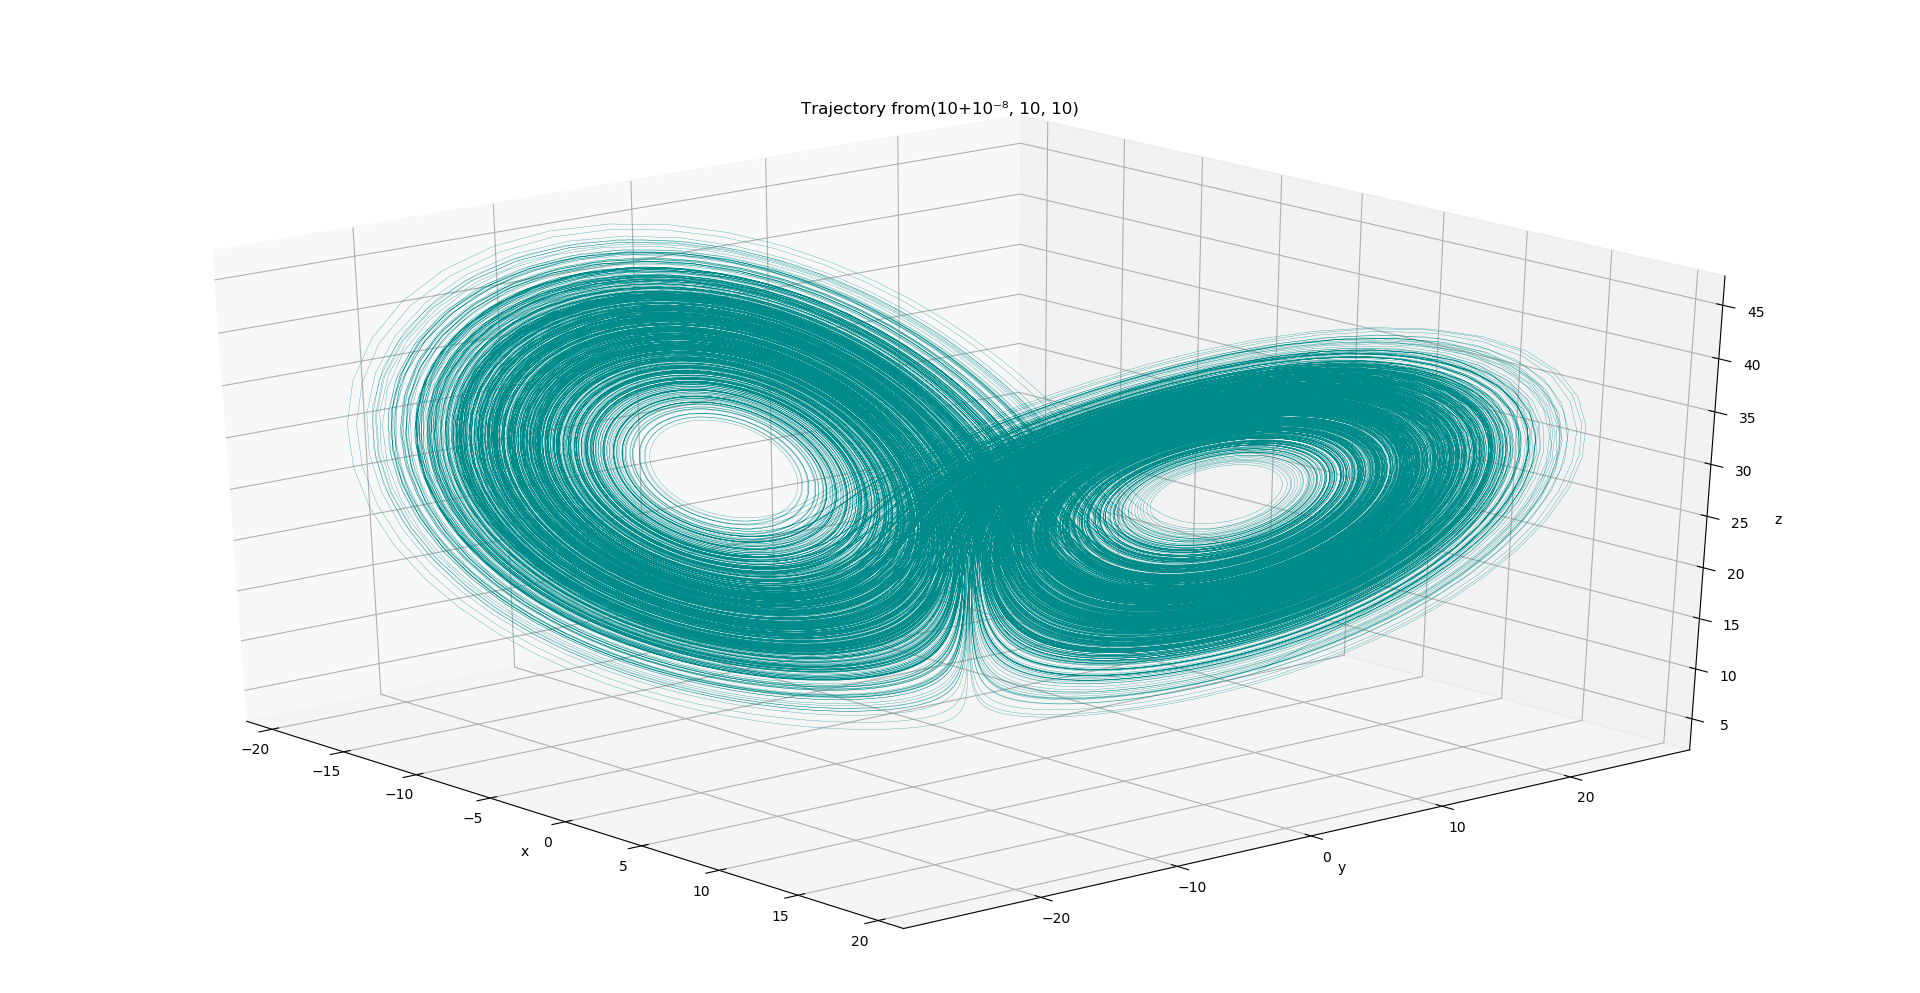
\includegraphics[width=0.7\textwidth]{../plots/lorenz_2.png}
    \caption{The trajectory of a Lorenz system with starting point $(10+10^{-8}, 10, 10)$.}
    \label{fig:lorenz_2}
\end{figure}

\begin{figure}[H]
    \centering
    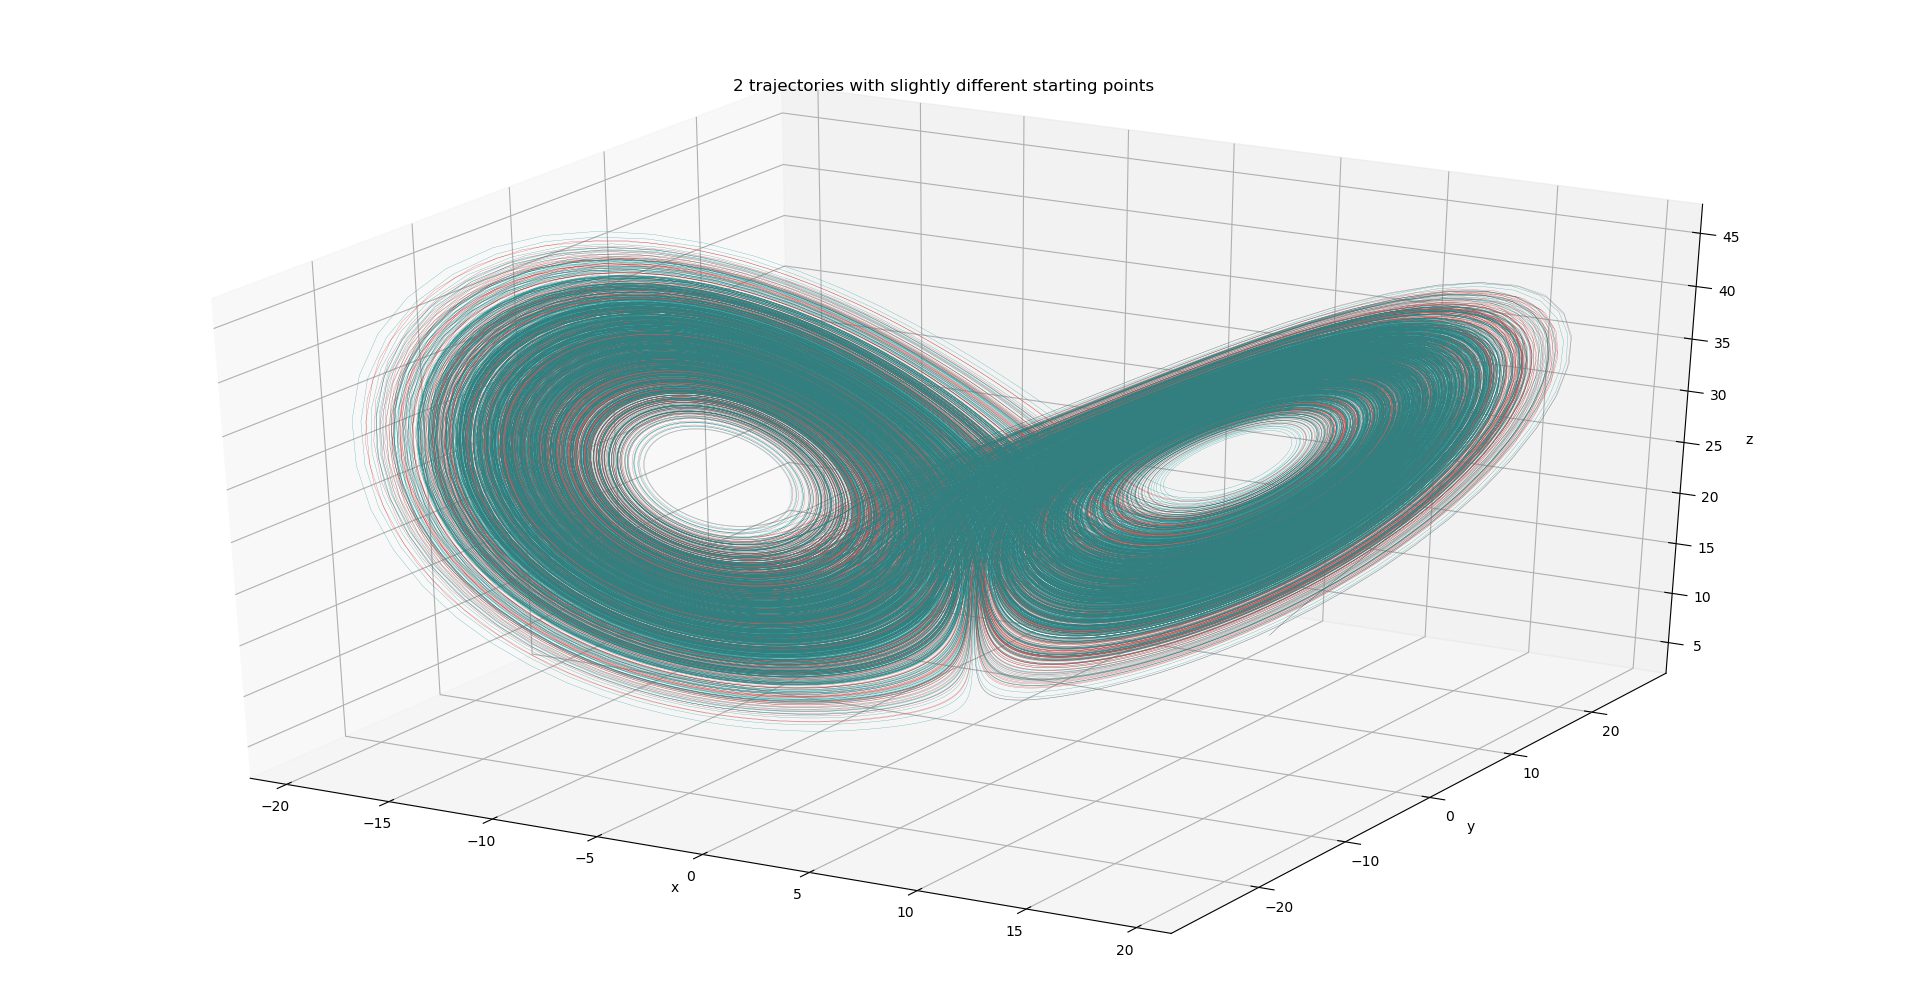
\includegraphics[width=0.7\textwidth]{../plots/lorenz_3.png}
    \caption{The trajectories plotted together with starting points $(10+10^{-8}, 10, 10)$ and $(10, 10, 10)$.}
    \label{fig:lorenz_3}
\end{figure}

If the $\rho$ parameter is changed to $0.5$, both of the trajectories with the aforementioned starting points converge to the same trajectory and end up roughly at the origin point as seen in Figure \ref{fig:lorenz_4}, which happens to be their steady state. Since $\rho=0.5$ has a steady state and $\rho=28$ does not, there must be a bifurcation in between where the system loses its stability. \\

\begin{figure}[H]
    \centering
    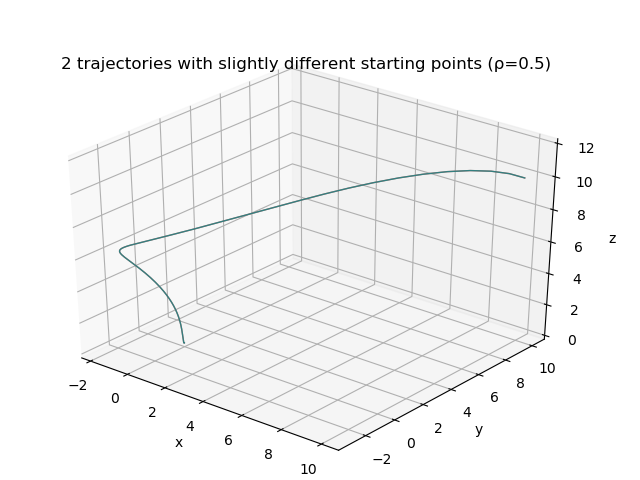
\includegraphics[width=0.7\textwidth]{../plots/lorenz_4.png}
    \caption{The trajectories plotted together with starting points $(10+10^{-8}, 10, 10)$ and $(10, 10, 10)$ where $\rho=0.5$. Both trajectories end up at origin.}
    \label{fig:lorenz_4}
\end{figure}

\end{task}
\begin{task}{5, Bifurcations in crowd dynamics}
First Part:
We have a given scenario for vadere, where one-hundred pedestrians are moving between two targets. In the middle between the two targets there is an obstacle, which affects the movement of the pedestrian according to its vertical position. The setup of the scenario can be seen in Figure \ref{fig:task5_setup}.
We run the scenario twenty-five times for different values of y which determinates the vertical position of the obstacle and consequently the movement of the pedestrians.
\begin{figure}[H]
\centering
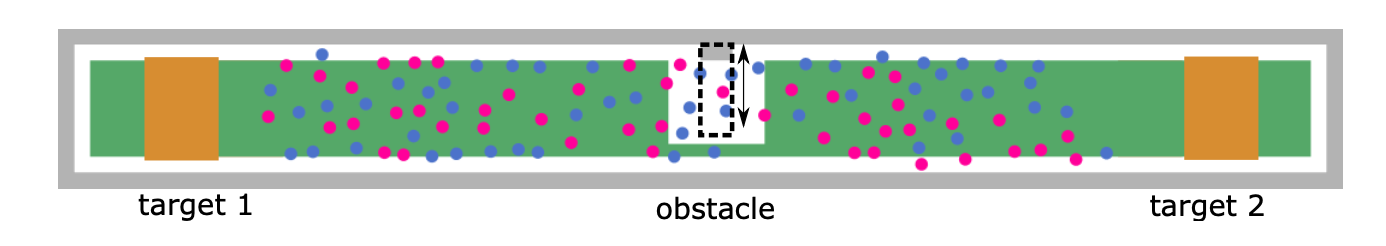
\includegraphics[width=0.7\textwidth]{../plots/scenario_setup.png}
\caption{Setup of the scenario for Task 5}
\label{fig:task5_setup}
\end{figure}
After running the simulation for vertical coordinates of the obstacle between 2.0 and 4.5, plots were generated showing the x and y coordinates for a single pedestrian for different scenarios. In case the obstacle is set only at the upper edge of the scenario, the pedestrians are barely affected and can move between both targets. This movement is visualized in Figure \ref{fig:task5_obstacle_up}. It can be seen that x-coordinate changes a lot for the pedestrian because he is walking from one target to the other, but the y-coordinate is not changing much.
\begin{figure}[H]
\centering
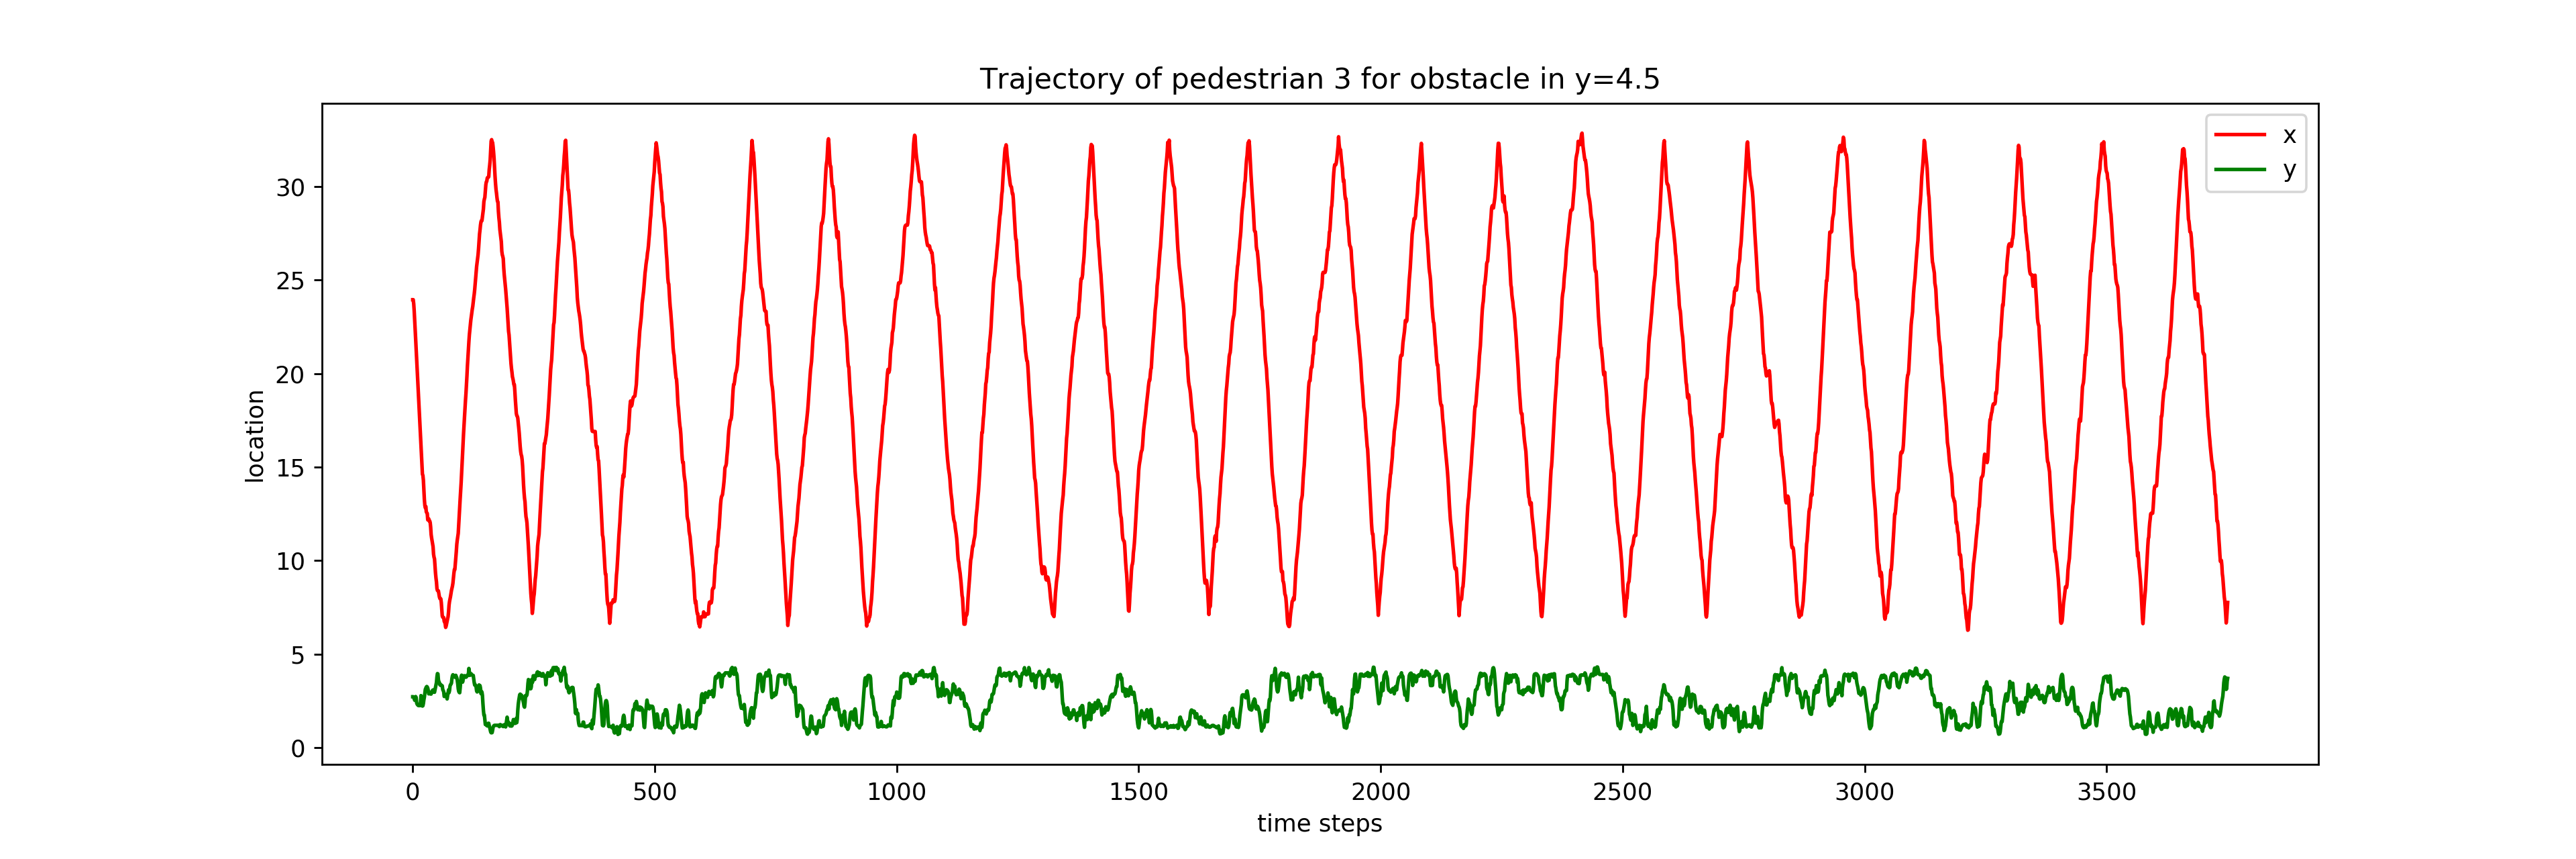
\includegraphics[width=0.7\textwidth]{../plots/task5/3_4,5.png}
\caption{Coordinates for pedestrian 3 for a vertical value of 4.5 of the obstacle}
\label{fig:task5_obstacle_up}
\end{figure}
In comparison to Figure \ref{fig:task5_obstacle_up} Figure \ref{fig:task5_obstacle_down} shows the coordinates of a pedestrian when the obstacle affects the movement a lot, because the vertical value of the obstacle is low and consequently the obstacle is set in the middle of the scenario. The pedestrian starts walking normally but stops already before timestep 500 is reached. The obstacle affects the movement so much that the pedestrians get stuck and the pedestrian of Figure \ref{fig:task5_obstacle_down} stays at the same position until the end of the simulation. This can be seen that neither the x nor the y coordinate are changing after timestep 500.
\begin{figure}[H]
\centering
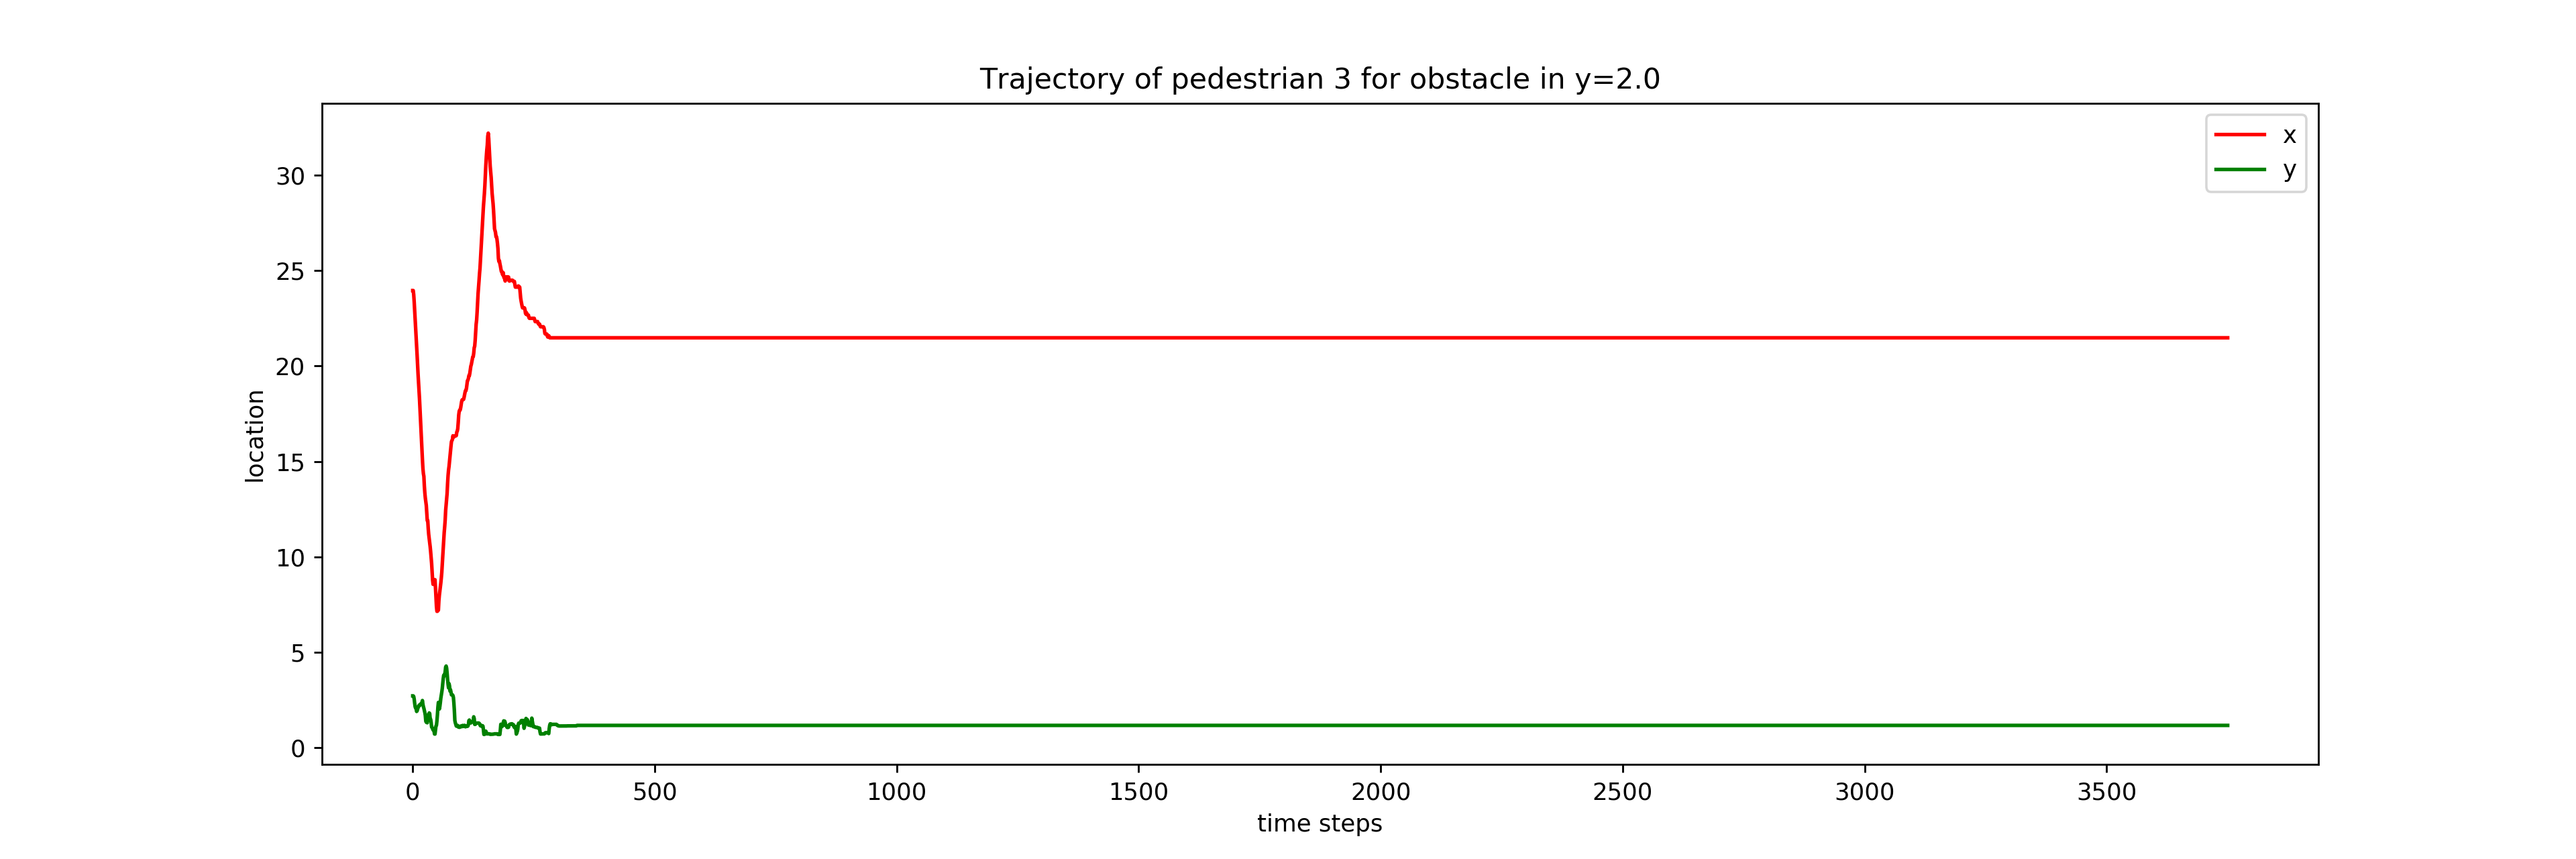
\includegraphics[width=0.7\textwidth]{../plots/task5/3_2,0.png}
\caption{Coordinates for pedestrian 3 for a vertical value of 2.0 of the obstacle}
\label{fig:task5_obstacle_down}
\end{figure}
The 12th pedestrian and a time gap of 95 were chosen to plot the phase portraits. The time gap were chosen such that when x is at the bottom $x+t$ is at the next peak at the best case $(y=4.5)$. Some phase portraits of pedestrian 12 for various y values can be seen in Figures \ref{task5_phase2.7}, \ref{task5_phase3.5}, and \ref{task5_phase4.5}.\\
The minor principal component of the reduced phase portrait for $y=4.5$ was determined using Principal Component Analysis and was used to analyse possible bifurcations throughout all y values. The points of the graphs are projected onto that same principal component for each phase portrait and the change of standard deviations was plotted. As seen in Figure \ref{task5_std_change}, the standard deviation keep a steady and slight linear increase for $y\geq 3$; however, the change of standard deviation has no pattern for $y<3$ indicating a lack of steady state. Thus, it can be argued that a bifurcation occurs at y value of around 3.\\
\begin{figure}[H]
\centering
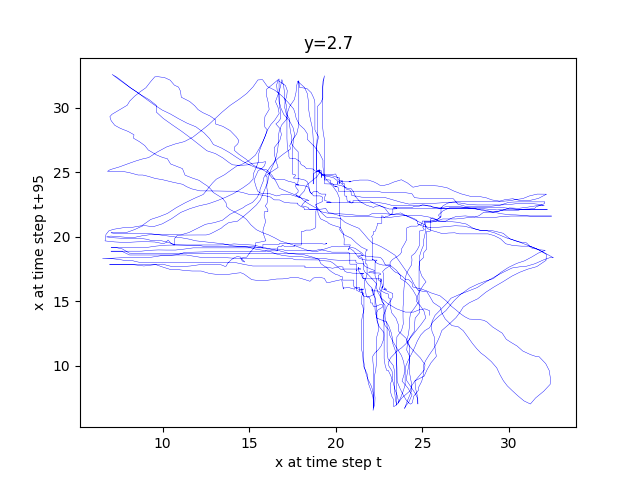
\includegraphics[width=0.7\textwidth]{../plots/task5/12_phase_portrait_y_2,7.png}
\caption{Phase diagram for pedestrian 12 for $y=2.7$}
\label{task5_phase2.7}
\end{figure}
\begin{figure}[H]
\centering
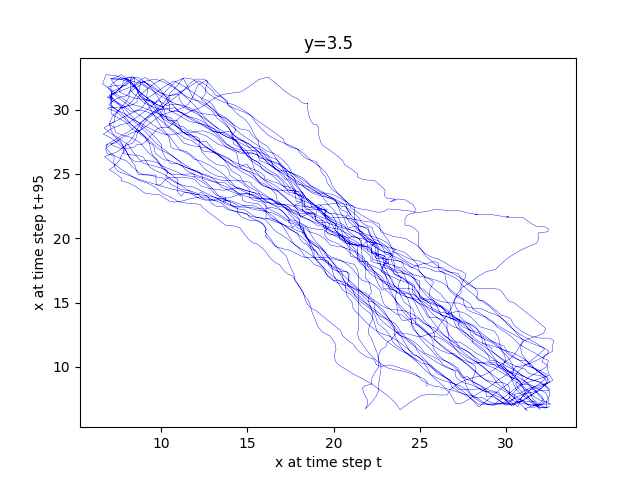
\includegraphics[width=0.7\textwidth]{../plots/task5/12_phase_portrait_y_3,5.png}
\caption{Phase diagram for pedestrian 12 for $y=3.5$}
\label{task5_phase3.5}
\end{figure}
\begin{figure}[H]
\centering
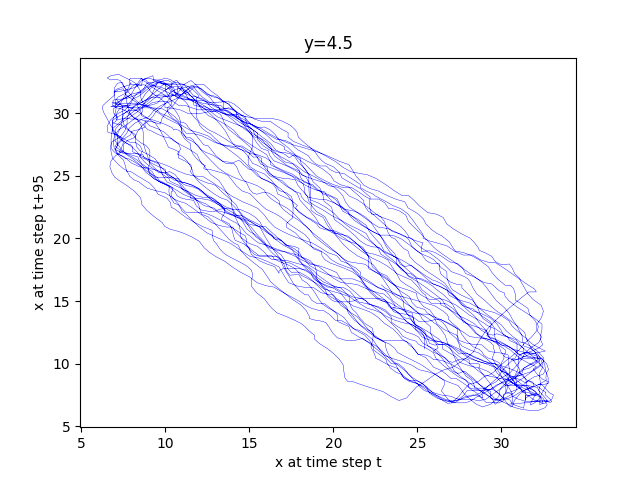
\includegraphics[width=0.7\textwidth]{../plots/task5/12_phase_portrait_y_4,5.png}
\caption{Phase diagram for pedestrian 12 for $y=4.5$}
\label{task5_phase4.5}
\end{figure}
\begin{figure}[H]
\centering
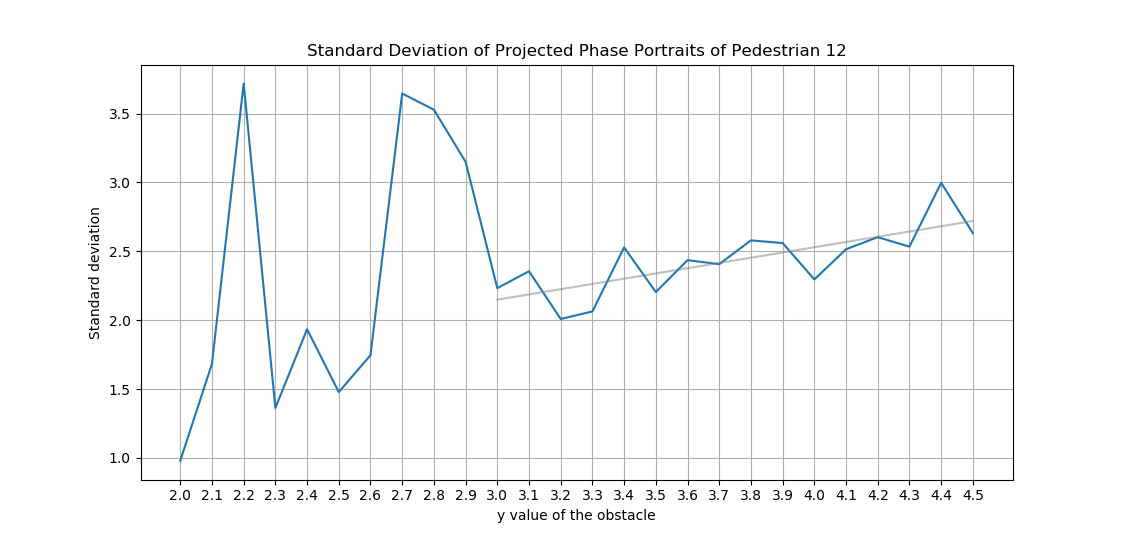
\includegraphics[width=\textwidth]{../plots/task5/std_projection_phase_ped12.png}
\caption{Change of standard deviation of projected phase portraits by y position of the obstacle.}
\label{task5_std_change}
\end{figure}
\bigbreak
Second Part:
For the second part, we came up with the following scenario which represents saddle node bifurcation. A source is set to be a certain distance away from two targets, on the x-axis. A parameter $d$ determines the distance between the targets As the distance cannot be negative so at $d < 0$, the behavior is not defined. At $d=0$, both of the targets are overlapping each other. So the pedestrians move from the source to the targets. As the becomes, $d > 0$, the targets move away from each other, at the rate of $\sqrt{d}$. For simplicity we consider a single pedestrian which moves from the source towards the targets. In each iteration depending upon initialized location of the pedestrian, it can move towards any of the two targets.
\textbf{Second Part:} \\
For the second part, we came up with the following scenario which represents saddle node bifurcation. A source is set to be a certain distance away from two targets, on the x-axis. A parameter $d$ determines the distance between the targets As the distance cannot be negative so at $d < 0$, the behavior is not defined. At $d=0$, both of the targets are overlapping each other. So the pedestrians move from the source to the targets. As the becomes, $d > 0$, the targets move away from each other, at the rate of $\sqrt{d}$. For simplicity we consider a single pedestrian from now on, which moves from the source towards the targets. In each iteration depending upon initialized location of the pedestrian, it can move towards any of the two targets.\\

The scenario depicts a saddle node bifurcation as, at values $d < 0$, no fixed point exists for the pedestrian to move towards. There is one fixed point at $d = 0$, i.e the overlapping targets and at $d > 0$, two fixed points exist and the pedestrian can move to any one of them. The distance between the targets increases as a function of $\sqrt{d}$, hence the fixed points always exist at $x_{0}=\sqrt{d}$. We could not simulate the stability of the two fixed points, because to be able to simulate the stability, one of the targets have to the attractor and the repeller but we could not find the functionality of a repeller in Vadere software. \\

One of the examples of a system with saddle node bifurcation is: \\
\begin{center}
$\frac{dx}{dt} = r + x^{2}$
\end{center}

This is the normal form of saddle node bifurcation. A differential equation $\frac{dx}{dt} = f(r, x)$ with a fixed point at $x=0$ for $r=0$ with $\frac{\partial f}{\partial x}(0, 0) = 0$ is topologically equivalent to the normal form of saddle node bifurcation provided the conditions of nondegeneracy, i.e. $\frac{\partial^2 f}{\partial x^2}(0, 0) \neq 0$ and transversality i.e. $\frac{\partial f}{\partial r}(0, 0) \neq 0$. 

\begin{figure}[H]
    \centering
    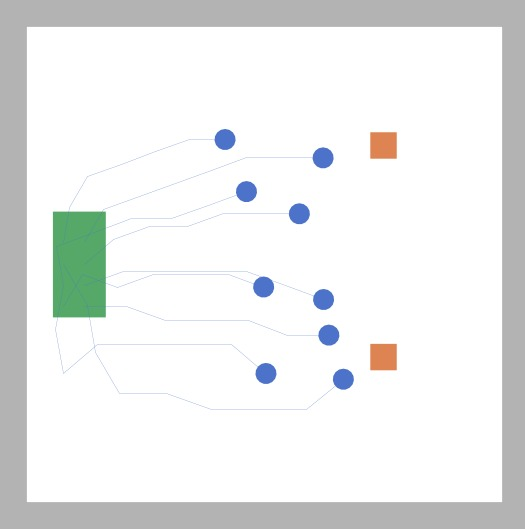
\includegraphics[width=0.5\textwidth]{./pictures/task5_2.jpeg}
    \caption{The scenario with two targets and a source.}
    \label{fig:task5_2}
\end{figure}

\begin{figure}[H]
    \centering
    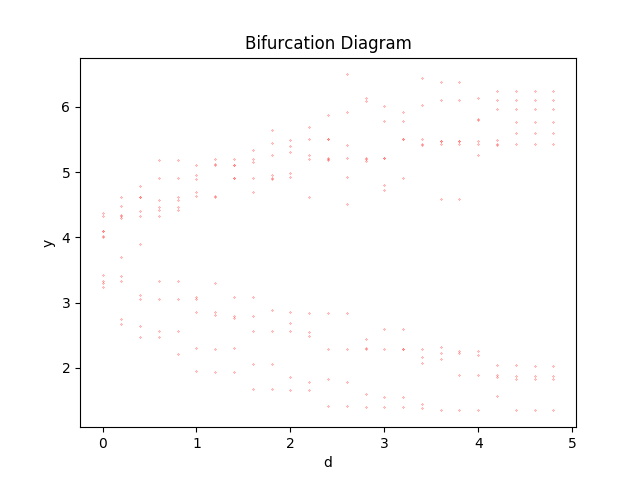
\includegraphics[width=0.7\textwidth]{../plots/task5/saddle_bifurcation.png}
    \caption{The bifurcation diagram for the proposed scenario. The stable and unstable overlay shows the expected plot according to saddle node bifurcation}
    \label{fig:part2_bifurcation}
\end{figure}

\begin{figure}[H]
    \centering
    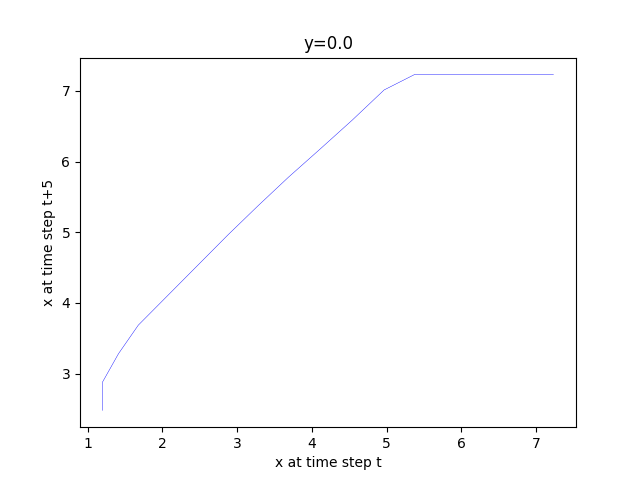
\includegraphics[width=0.7\textwidth]{../plots/task5/0_phase_portrait_y_0_0_second_part.png}
    \caption{The phase portrait at d = 0.0}
    \label{fig:part2_bifurcation}
\end{figure}

\begin{figure}[H]
    \centering
    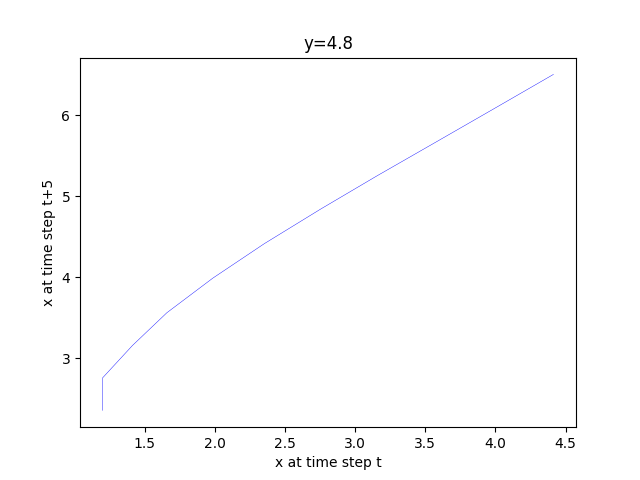
\includegraphics[width=0.7\textwidth]{../plots/task5/0_phase_portrait_y_4_8_second_part.png}
    \caption{The phase portrait at d = 4.8}
    \label{fig:part2_bifurcation}
\end{figure}
As it can be deduced from the bifurcation diagram that the scenario explained in this part can be represented by the following differential equation:
\begin{center}
	$\frac{dx}{dt} = r + x^{2} + 4$
\end{center}
It can be proven with simple calculus that the two conditions for the saddle node bifurcation holds on this dynamical system.
\end{task}
\newpage
\bibliographystyle{ieeetr}
\bibliography{report}
\nocite{*}
\end{document}
